\chapter{Unimodal Black-box Models}\label{chapter:uni_modality}
\textit{``Prediction is very difficult, especially if it's about the future''}-
Niels Bohr

\section{Chapter Overview} 
CNVs is one type of omics data that are defined as the segment of DNA 41 kb in size~\cite{almal2012implications}. Research has exposed that many of the genes~(especially, cancer-related genes) are disrupted by a CNV~\cite{almal2012implications}. This chapter focuses on single input modality CNV data to assess how accurately and confidently we can reveal the association of copy number variations~(CNVs) with cancer, a partial effort to develop a decision support system~(DSS) to answer the first research question\footnote{\textbf{RQ1}: \textit{How can multimodal data be more effective than unimodal data to provide accurate decision?}}. 
Through several experiments, a hypothesis will be built upon whether CNVs provides sifficient signals for cancer type classification. If yes, which classifier between CAE classifier and CLSTM is more suited. Knowing these will justify if CNVs should be considered an useful modality in multimodality integration in \cref{chapter:multiodality}. 

\hspace*{3.5mm} To establish this, first, CNV data covering 14 different cancer types from The Cancer Genome Atlas~(TCGA)~\cite{tcga}, will be used in order to create two different training sets will be prepared based on oncogenes and protein-coding genes. Then two neural network architectures called convolutional-LSTM~({CLSTM}) and convolutional autoencoder classifier~({CAE}) are trained on both representations, followed by creating their snapshots models. %{CLSTM} and {CAE} are trained to capture important~(both locally globally) and abstract features, respectively. 
Finally, model averaging ensemble is applied to combine the predictions of snapshot models in order to provide diagnosis decision w.r.t cancer types. 

\section{Introduction}
With the high-throughput next-generation sequencing technologies, cancer-specific genetic profiling is now possible~\cite{tomczak2015cancer,tcga}. The entire genome sequencing data can be used to identify similar genetic mutations and genetic variations associated with different tumors~\cite{82Tomczak}. 
Variations in human genomic DNA make an individual unique in terms of disease susceptibility and response to certain drugs~\cite{almal2012implications}. 
%Discovery of biologically significant biomarkers is an important step in understanding the molecular mechanisms of carcinogenesis. An accurate diagnosis requires both omics data and clinical outcomes need to be analyzed, which is specific to patients with particular genomic profiles and molecular traits. 
However, one of the main challenges remain is to identify meaningful differences in the genomic information between individuals~\cite{almal2012implications}. 
Compared to reference genome, CNVs  vary in its copy number, making them bound to have vital role in disease susceptibility and drug response~\cite{almal2012implications}.
Besides, CNVs are found to be associated with the risk of cancer. 
Yuan et al.~\cite{yuan2018cancer} exposed that  CNVs are not only associated with complex diseases, but also contribute to growth of different types of cancers, e.g., CNVs are associated with the risk of pancreatic cancer~\cite{66Huang}). Calcango et al.~\cite{67Calcagno} studied copy number changes by comparing healthy vs. cancer patients, and found that amplification and deletion of certain genes are more common in some cancer patients. Therefore, accurate identification of biologically relevant genes can help reveal genetic predispositions before a certain cancer grows. Deletions and duplication in the cancer-related genes~(also called INDELS) are found to be polymorphic in different population. 

\begin{figure*}
	\centering
	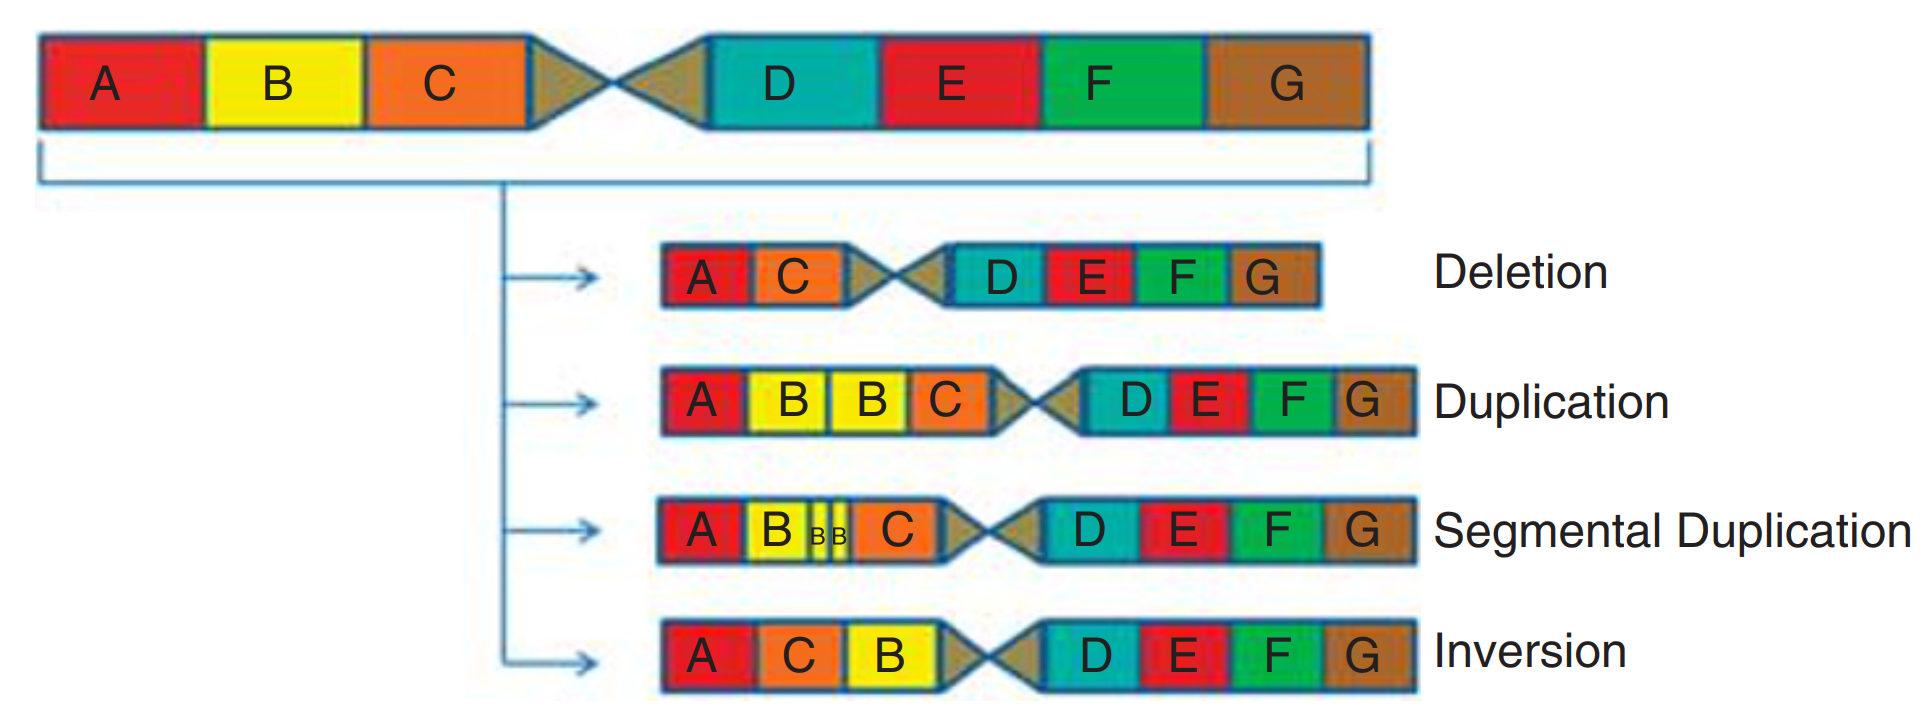
\includegraphics[scale=0.5]{images/cnv_v1.png} 
	\caption[Copy number variations, showing deletion, duplication, and inversion]{CNVs is classified into deletion, duplication, segmental duplication and inversion. These variations can affect an entire gene or a segment of a particular gene~\cite{almal2012implications}}	
	\label{fig:cnv_v1}
	\vspace{-2mm}
\end{figure*}

\hspace*{3.5mm} Besides, several biomarkers through single nucleotide polymorphisms~(SNP) studies have revealed an association with cancer and many other complex traits~\cite{almal2012implications}. An accurate identification of cancer based on CNVs can help to reveal the genetic predisposition for cancer before cancer actually occurs, so that vigilant prevention and rigorous monitoring may be practiced by those who are highly predisposed~\cite{19Cruz}. Inspired by this, CNVs were used to identify minimum redundancy maximum relevance feature selection and incremental feature selection methods~\cite{zhang2016classification} such that only one sample could be covered at a time or using microarray-based comparative genomic hybridization methods. Extracted CNVs features are then used to train machine learning~(ML) models for cancer identification, e.g., type prediction. Cancer typing methods based on manual feature selections and ML classifiers often involved inefficiency feature selection process using principal component analysis~(PCA) or recursive feature selection~\cite{malekpour2018mseq}. %, making them incapable for multiple samples and recurrent CNVs~\cite{malekpour2018mseq}. 

\hspace*{3.5mm} Nevertheless, genomics data, including CNVs, from TCGA show several characteristics~\cite{lu2003cancer} such as high dimensionality~(e.g., up to tens of thousands of genes), very small sample size~(e.g., less than $100$ samples), very sparse feature space~(e.g., as majority of genes are not responsible for cancer, making them irrelevant to cancer types classification). With such a huge feature space, even a robust ML model would fail to model the high-order non-linear interaction between biomarker genes. These characteristics make the overall analysis very challenging for  linear ML and tree-based models. ML-based approaches often fail to handle high dimensional and to model high-order interaction between a large number of biomarker genes. Besides, tree-based models are prone to overfitting, due to small sample size~\cite{lu2003cancer}. Since most genes are irrelevant for class distinction, their inclusion would not only introduce noise, but also trivial on-linearity~\cite{lu2003cancer}. Automated and robust feature selection and ranking of biologically meaningful biomarkers prior to classification help to mitigate these problems. 

\hspace*{3.5mm} In comparison with ML-based approaches, deep learning~(DL) approaches based on neural networks~(DNN), found to be effective. While convolutional neural networks~(CNN) is good at reducing frequency variations, long short-term memory~(LSTM) is good at modeling temporal and complex interactions between CNVs across genes. Further, a neural ensemble method is found to be more effective than structures solely based on CNN or LSTM. This chapter, focuses on CNVs-based cancer typing method~(i.e., single modality). We use MSeq-CNV~\cite{malekpour2018mseq} - a CNV feature extraction tool to extract recurrent CNVs~(i.e., including genomic deletions and duplication across samples). MSeq-CNV uses mixture density for modeling aberrations in depth of coverage and abnormalities in the mate pair insertion sizes. However, common CNVs across multiple samples can be detected. Since CNVs are very high dimensional, modelling non-linear interactions between oncogenes and protein-coding genes is very challenging. This chapter hypotheses the following to address above challenges: 

\begin{enumerate}[noitemsep]
    \item High dimensionality of genomic data\footnote{\textbf{H1}: Stacking and neural representation learning can be very effective at extracting most abstract features from high dimensional genomic data through a hierarchical learning process.} can be handled by learning most abstract features through a hierarchical learning process by stacking DNN architectures and neural representation learning. 
    \item A neural ensemble method\footnote{\textbf{H2}: A neural ensemble method by combining several deep architectures can be more effective than structures solely based on a single architecture by reducing generalization error}, by combining several deep architectures can be more effective than structures solely based on a single architecture by reducing generalization error.
\end{enumerate}

\hspace*{3.5mm} Based on these hypotheses, both {CLSTM} and CAE networks were trained and evaluated separately. Predictions of multiple model snapshots are then combined based on model weighted averaging ensemble of the classifiers\footnote{Supporting publication: \textbf{Md. Rezaul Karim}, Stefan Decker, and Oya Beyan, ``A snapshot neural ensemble method for cancer type prediction based on copy number variations", \emph{Neural Computing and Applications}, November 30, 2019.}.  %Further, we provide interpretations about the prediction made by the neural network in order to make the cancer diagnosis more effective. 
The rest of the chapter is structured as follows:
\cref{chapter_3:rw} covers some related works concerning cancer diagnosis based on CNVs data and summarizes their potential limitations. \Cref{chapter_3:mm} chronicles the detail of the data collection and feature engineering before the network construction and training. \Cref{chapter_3:results} demonstrates some experimental results and discusses key findings of the study. \Cref{chapter_3:conclusion} provides explanations of the importance and relevance of the study reported, highlights potential limitations, and discuss some future works before concluding the chapter. 

\section{Related Work}\label{chapter_3:rw}
As shown in \cref{table:stateofart}, both genomic, bioimaging, and clinical outcomes~\cite{min} are used to provide accurate diagnosis. In particular, RNA-Seq data is more widely used to identify rare and common transcripts, isoforms, and protein-coding RNAs in cancer. Single nucleotide polymorphism data used to identify segmental variations across multiple cancer genomes~\cite{82Tomczak,95Gaul}). Ning Z. et al.~\cite{zhang2016classification} used CNVs level from cBioPortal for Cancer Genomics\footnote{cBioPortal for Cancer Genomics: \url{https://www.cbioportal.org/}}~\cite{cerami2012cbio} to classify the patients into breasts, bladder urothelial, colon, glioblastoma, head and neck squamous cell, and kidney cancer types. They construct a dagging-based classifier where the feature space was reduced using minimum redundancy maximum relevance feature selection and incremental feature selection methods~\cite{zhang2016classification}. They achieved an accuracy of 75\%, indicating that mostly driver genes play key role in differentiating cancer types. 

\hspace*{3.5mm} Sanaa et al.~\cite{elsadek2018supervised} extended their work in which 7 ML classifiers were trained giving the random forest algorithm an accuracy of 86\%. Other works used omics data to identify various cancer types e.g., Fakoor et al.~\cite{fakoor} extract features from high dimensional GE data using PCA and classify them into acute myeloid leukemia, breast, and ovarian cancer patients. Besides, CNVs analysis based on different statistical methods also used to identify significant CN associated with different types of cancers~\cite{cancernet}. Fisher's exact test is applied on patient and control groups to identify copy numbers for hereditary breast and ovarian cancer~\cite{58Kuusisto}. Although Fisher's exact test is mainly used for CNV analysis~\cite{fish}, ML-based approaches are trending to improve the accuracy of cancer susceptibility, recurrence, and survival prediction~\cite{16Kourou}. However, accurate extraction of CNVs and dealing with dimensionality remain two key challenges. ML algorithms such as support vector machine~(SVM) and decision trees are found effect to extract the most significant CNVs features from high dimensional data. 

\hspace*{3.5mm} In comparison with ML-based approaches, recent DL techniques have shown more accurate and promising results for cancer identification in some studies. CNN is widely applied~\cite{19Cruz} on whole slide images in order to detect cancer regions with a very high degree of precision, which is mainly because CNN can extract deep features from different cohorts simultaneously. Ibrahim et al.~\cite{ibrahim} proposed a multilevel feature selection technique based on deep belief networks and unsupervised active learning from miRNA expression data, which outperforms PCA-based methods for hepatocellular and breast carcinoma identification. Danaee et al.~\cite{17Danaee} used stacked denoising autoencoder to extract features from the RNA-seq data, which are then fed into SVM and shallow neural network to classify the samples into malignant or benign tumor of breasts~\cite{18Chen}. DeepCNA is another CNN-based approach proposed by Yuan et al.~\cite{yuan2018cancer} for cancer type prediction based on CNVs and chromatin 3D structure. DeepCNA performs moderately well if both CNA and 3D chromatin structures are used in a multimodal setting, which is, however, not always possible in a resource constrained setting. % for genomics-based cancer detection. 

\hspace*{3.5mm} Besides, imaging modalities such as histology and radiological images are used for understanding the genetic and epigenetic causes of cancer~\cite{20Rajanna,23Zheng} and to identify the existence of cancer using CNN~\cite{19Cruz,xu}. GISTIC and mutation significance\footnote{MutSig and GISTIC provide statistical significance of recurrence of mutations and copy-number alterations in specific genes, URL: \url{https://software.broadinstitute.org/cancer/cga/mutsig}} tools were employed to analyse the samples, followed by K-means clustering to visualize genomic and transcription alterations in various cancers~\cite{wb}. X-ray and CRT images are also used, along with proteomic and genomic assays which shows success in cancer prediction and prognosis~\cite{28Zhou}. Often these images are used to generate noninvasive, functional, and molecular multispectral photoacoustic imaging to detect prostate cancer using K-means and SVM~\cite{23Zheng}. %Besides, histopathology images are used . 
%Literature~\cite{17Danaee} used stacked denoising autoencoder to extract features from RNA-seq data and then fed into SVM and shallow ANN to classify malignant or benign tumor of breasts~\cite{18Chen}. DeepCNA is another CNN-based approach for cancer type prediction based on CNVs and chromatin 3D structure~\cite{yuan2018cancer}.
%Apart from these works, restricted methods have been proposed based on CNVs for cancer risk and type predictions~\cite{ding2014application, zhang2016classification, elsadek2018supervised}. 

\begin{table*}[!ht]
    \caption{Different cancer detection methods, data types, and performance }
    \label{table:stateofart}
    \begin{center}
    \scriptsize
    \vspace{-6mm}
    \begin{tabular}{l|l|l|l|l|l}
        \hline
        \textbf{Reference} & \textbf{Approach} & \textbf{Cancer types} & \textbf{\#Sample} & \textbf{Data type} & \textbf{Accuracy} \\\hline
            Karim et al.~\cite{karim2018a2ic} & DBN/LSTM & 14 primary types & 15,699 & TCGA CNVs & 73\% \\\hline % 2018
            Yuan et al.~\cite{yuan2018cancer} & CNN & 25 primary types & 14,703 & CNA \& 3D cromatin & 90\% \\\hline % 2018
            Sanaa et al.~\cite{elsadek2018supervised} & LR & 6 primary types & 3,480  & CNVs & 85\% \\\hline % 2018
        	Cruz et al.~\cite{19Cruz} & CNN & Breast cancer  & 605 & Slide images & 96\%  \\\hline  % 2017
            Danee et al.~\cite{17Danaee} & MLP & Breast cancer & 1210 & RNA-seq & 94\% \\\hline % 2016
            Ning et al.~\cite{zhang2016classification} & Dagging & 6 primary types & 3,480  & CNVs & 75\% \\\hline % 2016
        	Rajana et al.~\cite{20Rajanna} & Deep NN & Prostate cancer & 807 & Histology & 95\%\\\hline
            Chen et al.~\cite{18Chen} & Shallow NN & Colon cancer  & 590 & Gene expression & 84\% \\ \hline % 2015
            Ahmed et al.~\cite{abdel2016breast} & DBN & Breast cancer & 569 & Wisconsin BRCA & 99\% \\ \hline % 2015
            Zheng et al.~\cite{23Zheng} & K-means/SVM & Breast cancer & 569 & Wisconsin BRCA & 97.38\% \\ \hline % 2014
            Xiaofan et al.~\cite{ding2014application} & Naïve Bayes & Cancer risk & 640 & Human SNP & 93\% \\ \hline % 2014
        \end{tabular}
        \vspace{-6mm}
    \end{center}
\end{table*}

\hspace*{3.5mm} Unlike conventional cancer typing methods that work on analyzing morphological appearances, gene expression~(GE) levels of the tumor cells are used to differentiate tumors that have similar histopathological appearances~\cite{paroder2006na+}. Different types of somatic mutations data such as point mutation, single nucleotide variation~(SNV), small insertion and deletion\footnote{These are commonly known as INDELs}, copy number aberration~(CNA), translocation, and CNVs are also used. Xiaofan D. et al~\cite{ding2014application} extracted recurrent CNVs from non-tumor blood cell DNA of healthy patients. They revealed key the difference between cancer patients and controls w.r.t copy number losses and gains. Although their study can predict cancer predisposition of unseen test groups of mixed DNA with high confidence, a has limited coverage of only Caucasian and Korean cohorts. 

%\hspace*{3.5mm} Imaging data such as histology and radiological images are used for understanding genetic and epigenetic causes in cancer analyses~\cite{yuan2018cancer,20Rajanna,23Zheng}. In particular, GISTIC, MutSig, and clustering algorithms are used to visualize genomic and transcription alterations in various cancers at an advanced level~\cite{wb}. X-ray and CRT images~\cite{25Cruz}, along with proteomic and genomic assays, are also used, which show great success in cancer prediction and prognosis~\cite{28Zhou}. These types of images are used to generate noninvasive, functional, and molecular imaging modality data called multispectral photoacoustic imaging~\cite{20Rajanna} in order to detect prostate cancer using K-means and SVM~\cite{23Zheng}. 

%\hspace*{3.5mm} Literature~\cite{17Danaee} used a stacked denoising autoencoder to extract features from the RNA-seq data, which are then feed into SVM and shallow ANN to classify malignant or benign tumor of breasts~\cite{18Chen}. DeepCNA is another CNN-based approach proposed for cancer type prediction based on CNVs and chromatin 3D structure with CNN~\cite{yuan2018cancer}. Although DeepCNA is very efficient in cases where both CNA and 3D chromatin structures are supplied, the availability of such resources is not always possible, like in genomics-based cancer detection. Therefore, many researchers try to extract genomics data to be consumed by the DNN architectures. Apart from these works, restricted approaches have been proposed based on CNVs for cancer risk and type predictions~\cite{ding2014application, zhang2016classification, elsadek2018supervised}. Xiaofan D. et al.~\cite{ding2014application} used recurrent CNVs from non-tumor blood cell DNAs of non-cancer subjects about hepatocellular carcinoma, gastric cancer, and colorectal cancer patients. They revealed the differences between cancer patients and controls with respect to CN losses and CN gains. Although their study can make predictions on the cancer predisposition of an unseen test group of mixed DNAs with high confidence, it was limited to only Caucasian and Korean cohorts. 

%\hspace*{3.5mm} Ning Z. et al.~\cite{zhang2016classification} used CNVs at a level of 23,082 genes for 2,916 instances from cBioPortal for Cancer Genomics to classify 6 different types of cancers, i.e., breasts, bladder urothelial, colon, glioblastoma, kidney, and head-and-neck squamous cell. They construct a dagging-based classifier in which the feature space was reduced into CNVs of 19 genes using mRMR and IFS methods. They managed to achieve an accuracy of 75\%, indicating that only a few genes may play important roles in differentiating cancer types. Sanaa et al.~\cite{elsadek2018supervised} used the same dataset and train 7 different classifiers in which random forest shows 86\% accuracy. %The data used the CNV in variant types of cancers were downloaded from the

\hspace*{3.5mm} These approaches have not only proven to be useful at improving cancer diagnosis and subsequent treatments, but also revealed subtype information~\cite{66Huang}. Inspired by this, we considered copy number segmentation an important feature in a previous approach~\cite{karim2018a2ic}, such that higher the segmentation mean, the higher the copy number would be in that region. The length of a copy number and its value were then calculated based on a difference between start and end positions of a CNV. We represented copy number loss and gain in terms of negative segmentation mean and positive segmentation mean, respectively. Copy number with segmentation values between a certain range were considered as noise and discarded from rest of the calculation. However, a manual approach for CNV extraction like this often fails to extract recurrent CNV features in the case of simultaneous analysis of multiple samples~\cite{malekpour2018mseq}. Consequently, MSeq-CNV is applied for more efficient extraction of CNVs. 

%\hspace*{3.5mm} %\subsection{Related works on multimodality}
%Literature~\cite{liang} proposed to cluster ovarian and breast cancer patients based on multiplatform genomics~(e.g. GE, DNA methylation, and miRNA expression) and clinical data. To deal with such multiplatform data, MAE is used in which latent features are extracted before clustering with the K-means. Ngiam et al.~\cite{NgiamKKNLN11} proposed a multimodal architecture to handle multimodality of audio and video features based on three methods: multimodal fusion, cross-modality learning, and shared representation learning. 
%While each method uses multimodalities on the feature learning steps, multimodal fusion uses multimodalities in supervised learning and testing. Cross-modality learning used one type of data for both supervised learning and validating, while shared representation learning used one kind of data for supervised learning and testing. The original idea behind the cross-modality learning is to handle multimedia objects where not all data have all modalities. Liang et al.~\cite{liang} adopts a similar architecture for clustering multimodal cancer genomics GE, DNA methylation, and clinical data.

\section{Methods}\label{chapter_3:mm}
In this section, we discuss in detail the data collection, preprocessing, and feature engineering. % in detail. %, followed by the preparation of training, validation, and test sets. 

\subsection{Problem statement}
A CNV sample $x$ consists of a set of $m$ attribute-value pairs $\left(a_{i}, v_{i}\right)$, where $a_i$ is a feature and $v_i$ is its value from $a_{i}$, where both $a_{i}$ and $v_i \in \mathbb{R}^{D}$. %From given $n$ CNV samples $X$ = ${\{x_1,x_2, ..., x_n}\}$ in dataset $D$, where $x \in \mathbb{R}^{D}$. 
Let $X_{1}, X_{2}, \ldots, X_{m}$ be the CNV samples~(independent $m$-dimensional CNV samples~(i.e., $m$ is number of genes)) for the respective genes $G_{1}, G_{2}, \ldots, G_{m}$ respectively, where $X_{i} \in \mathbb{R}^{D}$ $\operatorname{dom}\left(X_{i}\right)$ which is the range of copy numbers for gene $G_{i}$. Let $C$ be the random variable for the class labels, and $\operatorname{dom}(C)=\{1, \ldots, K\},$ where $K$ denotes the total number of classes. If $t=\left\{t . X_{1}, t . X_{2}, \ldots, t . X_{m}\right\}$ denotes a size $m$ tuple of copy numbers for $m$ genes, $T=$ $\left\{\left(t_{1}, c_{1}\right),\left(t_{2}, c_{2}\right), \ldots,\left(t_{n}, c_{n}\right)\right\}$ denotes a training set of $n$ tuples, where $i=\{1,2, \ldots, n\}, c_{i} \in \operatorname{dom}(C)$ is the class label of tuple $t_{i} 
%Let the test set be $S=\left\{t_{1}, t_{2}, \ldots, t_{l}\right\}$ where $l$ is the size of the test set A classifier is a function Class with two arguments, $T$ and $s,$ where $T$ denotes the training samples and $s$ is a testing sample. Function Class returns a class prediction for sample $s .$ The classification accuracy is defined as the number of correct predictions made by the classifier on a set of testing tuples.
%Given a training set $T=\left\{\left(t_{1}, c_{1}\right),\left(t_{2}, c_{2}\right), \ldots,\left(t_{n}, c_{n}\right)\right\},$ where 
%$t_{i}$ are independent $m$-dimensional GE values~(i.e., $m$ is number of genes), 
=\left(t_{i} \cdot X_{1}, t_{i} \cdot X_{2}, \ldots, t_{i} \cdot X_{m}\right), m \gg n$ and $c_{i} \in \operatorname{dom}(\mathrm{C})$ is the class label of the $i^{th}$ tuple. 
First, we extract important features based on oncogenes and protein-coding human genes. 
Then we consider classifying an individual $x$ into a specific group or cancer type, where a predictor~(e.g., a classifier) is a function $F: {X}^{(m)} \rightarrow {Y}$, which maps the data instance from a feature space ${X}^{(m)}$ with $m$ input features to a labels $y$ in a target space ${Y}$, where $F(x)=y$ denotes the decision $y$, predicted by $F$. We also assume that $F$ is a `black-box' predictor, whose internal functioning is either unknown~(or partially known) or known but not interpretable by a human. 
 
%In \cref{chapter:uni_modality}, we developed a `black-box' predictor $f$ whose internal functioning is either unknown~(or partially known) to the observer or they are known but not interpretable by a human. In this chapter, instead we denote $\widetilde{f}$- an interpretable predictor, whose internal processing yielding a decision $\widetilde{f}(x)=y$ can be given a symbolic interpretation understandable by a human. %Examples of such predictors include rule-based classifiers, decision trees, decision sets, and rational functions. 

%the classifier $f$ maps an input $x$ to an output $f(x) \in y, f: \mathbb{R}^{d} \mapsto y$.

\subsection{Datasets}
\label{data}
Copy numbers and gene coordinates of different cancer types from TCGA are used in our study, which are hybridized by genome sequencing technology called {affymetrix SNP 6.0}, which allows us to examine the largest number of cases along with the highest probe density~\cite{31Park}. Tumor tissue and healthy tissue samples are collected from each cancer patient, which are curated from the blood, bone marrow, Buccal cell, EBV immortalized, and solid tissues. For consistency across samples, all data were downloaded from the same platform but with different project ID and gender. However, blood-derived healthy samples of only 14 cancer types were downloaded having at least 400 samples, as shown in~\cref{table:alldatadetails}. 

\begin{table} [!ht]
    \small
    \caption{Number of CNV samples across 14 different tumor types used in this chapter}
    \vspace{-2mm}
    \label{table:alldatadetails}
    \centering{
    \begin{tabular}{l|l|l|l}
        \hline
        \rowcolor{Gray}
         \textbf{Cohort} & \textbf{\#Tumor sample} & \textbf{\#Healthy sample} & \textbf{Carcinoma type} \\\hline
        COAD & 502 & 468 & Colon cdenocarcinoma \\\hline
        GBM  & 609 & 527 & Glioblastoma multiforme \\\hline
        KIRC & 586 & 530 & Kidney renal clear cell carcinoma  \\\hline
        LGG  & 514 & 487 & Brain lower grade glioma \\\hline
        LUAD & 554 & 591 & Lung adenocarcinoma \\\hline
        LUSC & 524 & 535 & Lung squamous cell carcinoma \\\hline
        OV   & 572 & 546 & Ovarian serous cystadenocarcinoma \\\hline
        UCEC & 548 & 545 & Uterine corpus endometrial carcinoma \\\hline
        BRCA & 1103 & 1103 & Breast invasive carcinoma  \\\hline 
        HNSC & 519 & 562 & Head \& neck squamous cell carcinoma \\\hline 
        THCA & 505 & 513 & Thyroid carcinoma \\\hline 
        PRAD & 501 & 536 & Prostate adenocarcinoma \\\hline 
        STAD & 442 & 464 & Stomach adenocarcinoma \\\hline 
        BLCA & 416 & 397 & Bladder urothelial carcinoma \\\hline
    \end{tabular}}
    \vspace{-2mm}
\end{table}

\iffalse
\begin{table} [h]
\centering
    \scriptsize
    \caption{number of CNV samples across 14 different tumor types}
    \label{table:alldatadetails}
    \vspace{-2mm}
    \begin{tabular}{l|l|l|l}
        \hline
        \rowcolor{Gray}
         \textbf{Cohort} & \textbf{DNA methylation} & \textbf{Copy numbers} & \textbf{Mutations} & \textbf{miRNA} & \textbf{Gene expression} & \textbf{Carcinoma type} \\\hline
            LUSC & 358 & 345 & 178 & 332 & 227 & Lung squamous cell carcinoma \\\hline
            READ & 162 & 164 & 69 & 143 & 71 & Rectum adeno-carcinoma \\%
            GBM  & 405 & 578 & 290 & 501 & 495 & Glioblastoma multiforme \\\hline
            LAML & 194 & 198 & 197 & 187 & 179 & Acute myeloid leukemia	\\%
            HNSC & 310 & 310 & 277 & 309 & 303 & Head \& neck squamous cell carcinoma \\\hline 
            BLCA & 126 & 126 & 99 & 121 & 96 & Bladder urothelial carcinoma \\\hline 
            KIRC & 457 & 457 & 417 & 442 & 431 & Kidney renal clear cell carcinoma  \\\hline
            UCEC & 512 & 511 & 248 & 497 & 333 & Uterine corpus endometrial carcinoma \\\hline
            LUAD & 431 & 357 & 229 & 365 & 355 & Lung adenocarcinoma \\\hline
            OV   & 592 & 577 & 316 & 454 & 581 & Ovarian serous cystadenocarcinoma \\\hline
            BRCA & 888 & 887 & 772 & 870 & 817 & Breast invasive carcinoma  \\\hline
            COAD & 420 & 422 & 155 & 407 & 192 & Colon cdenocarcinoma \\\hline
            %LGG  & 514 & 487 & Brain lower grade glioma \\\hline
            %THCA & 505 & 513 & Thyroid carcinoma \\\hline 
            %PRAD & 501 & 536 & Prostate adenocarcinoma \\\hline 
            %STAD & 442 & 464 & Stomach adenocarcinoma \\\hline 
    \end{tabular}
\end{table}

\fi 

\hspace*{3.5mm} We consider gender an important feature for cancer subtype classification, since tumors such as {BRCA} and {OV} are not common in males, whereas {PRAD} is only common in males. TCGA do not specify if a sample is curated from healthy tissue or tumor tissue, so we downloaded CNV files in separate groups. Each cancer sample is then grouped as primary and blood-derived samples during filtering before dividing them into male and female groups. We also used gene locations in combination with the copy number data, which are available in all patients for each tumor under each TCGA project. Gene coordinates were collected from cytobands using the ensemble library of \texttt{biomaRt} package\footnote{\url{https://www.ensembl.org/biomart}}. Additionally, oncogenes information were downloaded\footnote{TCGA has listed 568 oncogenes till September 2017} from the TCGA portal. 
%An example of a raw sample of GBM tumor is given in \cref{cnv:gbmCNV2}. 
%Each row in the table represents copy number changes at a specific DNA segment. For example, there is a copy number gain in the first row, which is from location 61,735 to 28,43676 in chromosome 1. However, only 557 probes being used to identify this segment change, which is quantified to 0.0548. Negative segment change represents the deletion from that region. 

\hspace*{3.5mm} Initial prepossessing were required to remove noise, empty, or string values from both CNV and gene data. For each cancer type, samples were downloaded into four different groups: healthy samples from male, healthy samples from female, tumor samples from male, and tumor samples from female. Then we preprocessed CNV data for 15,699 separate samples. Then, all the cancer samples and healthy tissue samples were combined. We found that the distribution of copy numbers across tumor samples are very different. For example, BRCA has almost double the samples of most other tumors. Whereas, {STAD} and {BLCA} have fewer samples compared to other tumor samples except for those having samples between 500-600. While, more than 400 THCA samples have 50 to 100 CNVs per sample, and around 50 OV tumor samples have less than 200 CNVs per sample. 

\iffalse
\begin{table} [!ht]
    \vspace{-3mm} 
    \caption{Example of a COAD CNV sample after preprocessing}
    \label{sample:afterpreprocessing}
    \begin{center}
    \small
    \begin{tabular}{l|l|l|l|l|l|l|l}
    \hline
    \rowcolor{Gray}
    \textbf{Chr} & \textbf{Start} & \textbf{End} & \textbf{Length} & \textbf{Segment\_Mean} & \textbf{Gain/Loss} & \textbf{Gender} & \textbf{Type} \\\hline
        1 & 1710664 & 1741164 & 30500 & -1.2237 & 0 & 0 & 1 \\\hline
    	1 &	16577231 &	16637050 &	59819  & 0.4852 &	1 &	0 &	1  \\\hline
    	1 &	16684955 &	16721910 &	36955  & 0.7576 &	1 &	0 &	1  \\\hline
        1 &	16721984 &	16855942 &	133958   & -0.5558 &	0 &	0 &	1  \\\hline 
    \end{tabular}
    \end{center}
    \vspace{-3mm}
\end{table}
\fi 

\hspace*{3.5mm} Although, most tumor samples have copy numbers between 50-400, there are a few samples having more than 1,500, giving on average 226.80 copy numbers per sample. On average, 106.92 copy numbers exist per healthy sample, which is less than half of tumor samples. Usually, healthy human cells have very different copy numbers in terms of location, length, and number and vary in humans. This makes the CNVs of the human genome an utterly complex and dynamic structure. For a cancer-affected patient, this structure becomes even more complex and dynamic as the tumor grows. In general, healthy human cells have completely different copy numbers in terms of location, length, and number from another human. 

\hspace*{3.5mm} We solve this dynamic dimension problem by using gene locations of the human genome since DL models expect fixed dimension inputs only. We selected a fixed number of genes and extracted the copy numbers that overlapped with the gene locations, removing them from the protein protein-coding gene because arguably more than 80\% of human genes do not encode any protein. Thus, copy numbers from these regions have little-to-no effect on tumor growth. %By using gene locations, we safely removed copy numbers that fall within protein-coding regions and kept those copy numbers that only affect genes.
%In addition, since not all genes are available in every human body and vary from person to person, genes are also variable in the human genome. 
We prepared two different datasets of CNVs based on oncogenes and protein-coding genes that are used to train the CLSTM and CAE networks to get the ensemble from. Additionally, some preprocessed data\footnote{Based on a Master thesis I co-supervised with Dr. Oya Beyan: "Using Deep Neural Networks and Copy Number Variations for Cancer Detection", by Md. Ashiqur Rahman, Software Systems Engineering, RWTH Aachen University, 2018.} were reused. %Data co %\Cref{fig:pipeline} shows the overall processing pipeline of our proposed approach.

\subsection{Feature selection from protein-coding genes}
We used the CNVs of 20,308 protein protein-coding genes. Since not all of these genes are responsible for tumor growth, features from irrelevant genes make the CNV data unnecessarily complex. Neural networks then fail to converge the training, resulting in poor performance. Although using protein-encoding genes makes the dimension fixed, 95\% of the features will be empty across the samples (e.g., a sample with 500 CNVs has 19,808 empty features making empty features for 19,808 cases). Using gene locations adds two additional complexities evolved: the curse of dimensionality and sparsity. 

\hspace*{3.5mm} To solve these problems, we perform CNV analysis in combination with 568 oncogenes responsible for the majority of cancer types. While oncogenes are found to be related to tumor growth, it is not confirmed which other genes also responsible for its growth. In such a setting, consecutive genes with non-zero values represent copy number length, and negative or positive segmentation values represent loss and gain, respectively. We hypothesize that DNN will be able to identify those hidden non-linear features. 

\subsection{Feature selection from oncogenes}
There are structural variations in DNA where protein-encoding genes are not present, and these genes have no effect on tumor growth. One way to remove such unnecessary segments is by keeping only those copy numbers that fall within gene regions and discarding the rest using oncogenes, because oncogenes not only control the cell division but are also responsible for gene expression changes due to external or natural causes and could lead to the development of tumor at some point. Thus, by considering only 568 oncogenes, we prepared another CNV representation instead of taking the whole 20,308 genes. 

\hspace*{3.5mm} As stated earlier, the manual CNV feature extraction is not efficient, and the recurrent CNVs from multiple samples are often ignored, we used the MSeq-CNV tool, which is an efficient CNV extraction method. In order to model the number of mate pairs with aberration in the insertion size and Poisson distribution for emitting the read counts, MSeq-CNV applies the binomial distribution-based mixture density on each genomic position. This applies a mixture density for modeling aberrations in depth of coverage and abnormalities in the mate pair insertion sizes. After applying MSeq-CNV, genome-wide copy gain and loss regions are saved in a matrix form, where each row represents a different CNV call with its sample number, start position, end position, and copy number estimation.
 
 \iffalse
\begin{figure}[ht!]
    \centering
    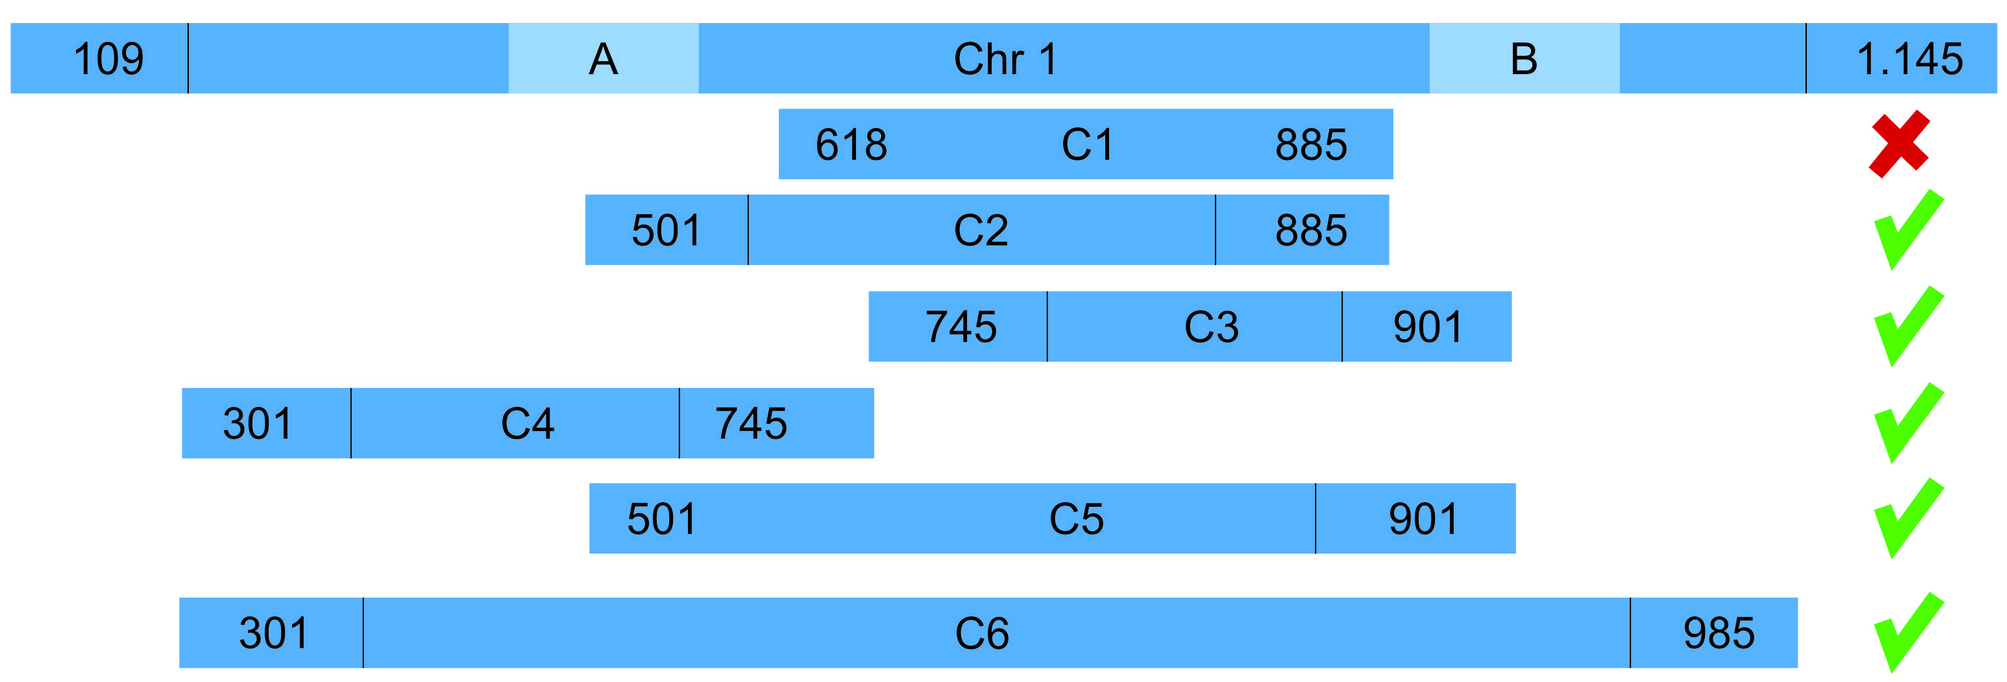
\includegraphics[width=0.90\textwidth,height=55mm]{images/fe.png}
    \caption{CNV selection process using MSeq-CNV}
    \label{fig:cnv_overlap}
\end{figure}
\fi 

%An example of the CNV selection process is shown in \cref{fig:cnv_overlap}. It shows a reference segment of chromosome 1 at the top that extends from DNA location 109 to 1,145 with two genes, A and B, within this segmental region. Below this reference, there are six candidate copy numbers~(C1-C6) at this location. C1 is a candidate copy number that extends between genes A and B, but C1 does not overlap with any one of them, which is why we remove it from the calculation. Candidates C2 and C3 are copy numbers, too, which slightly overlap with A and B, respectively. We still consider them as valid copy numbers because gene positions are not always fixed. C4 and C5 both fully overlap with genes A and B, hence, they are also valid copy numbers. C6 is not only a big segmental copy number, but it also overlaps with both genes. However, since we consider only the part of genes that overlap, we discard rest of the regions from the calculation. This is based on the hypothesis that even if a candidate copy number overlaps with a gene just by one base pair, we still consider it as a valid copy number~\cite{CNV2}. 

\vspace{-2mm}
\begin{table} [!ht]
    \caption{Example of training data prepared based CNVs representation of oncogenes}
    \label{cnv:changed232d}
    \vspace{-6mm}
    \begin{center}
        \scriptsize
        \begin{tabular}{l|l|l|l|l|l|l|l}
            \hline
            \rowcolor{Gray}
            \textbf{Type} & \textbf{Gender} & \textbf{PRDM16} & \textbf{RPL22} & \textbf{CAMTA1} & \textbf{MTOR} & .. & \textbf{MTCP1} \\\hline    
            COAD & 1 & -0.3195 & -0.2154 & 0 & 0.4767  & .. & 0.652 \\\hline
            PRAD & 0 & 0.230 & -0.552 & 1.715 & -0.92  & .. & -1.0 \\\hline
            OV & 1 & -1.240 & 0.975 & 0.350 & 0.642  & .. & 0.985 \\\hline
        \end{tabular}
        \vspace{-6mm}
    \end{center}
\end{table}
\vspace{-3mm}

\hspace*{3.5mm} Each gene has a starting and ending position in DNA, which is similar for copy numbers having starting and ending positions. For each gene, MSeq-CNV checks if a sample has any CNV region overlaps with that gene. Then it assigns the segment value for that gene, otherwise 0 is assigned. This means that a tumor sample has different copy number variation than a reference, which is measured by the segment value. If the value is positive, copy number in that gene is considered to be more increased than the reference. A negative value, however, signifies that the gene was deleted from that DNA location. A sample of the final training data is shown in table \ref{cnv:changed232d}. The first row shows a male patient's GBM tumor sample, where gene PRDM16 and RPL22 have copy number losses with segmentation values of 0.3195 and 0.2154, respectively. Whereas, gene CAMTA1 has no copy number variation, and so on. %Eventually, dimension of the training set reduced from 20,308 to 568 (+ the label column). 

\subsection{Network construction and training}
\label{nc}
We construct and train CLSTM and CAE networks on two different CNVs representations~(i.e., oncogenes and protein-coding genes), followed by the creation of multiple snapshot models. Then we evaluate each network independently, followed by the MEA to combine the snapshot models. 

\subsubsection{Construction of CLSTM network }
We construct and train the CLSTM network by combining both CNN and LSTM layers as shown in \cref{fig:conv_lstm}. While the CNN model uses conv filters to capture local relationship values, an LSTM network can carry overall relationship of a whole CNV sequence more efficiently. This turns CLSTM into a powerful architecture to capture long-term dependencies between features extracted by CNN~\cite{karim2019drug}. To capture both the local and global relationships, all the input ${X}_{1},{X}_{2},...,{X}_{t}$ cells in CLSTM output ${C}_{1},{C}_{2},...,{C}_{t}$, hidden states ${H}_{1},{H}_{2},....,{H}_{t}$, and gates $i_t$,$f_t$,$o_t$ of the network as 3D tensors whose last two dimensions are spatial dimensions. %To get a better picture of the inputs and states, we may imagine them as vectors standing on a spatial grid. 
CLSTM determines the future state of a certain cell in the input hyperspace by the inputs and past states of its local neighbors, which is achieved by using a convolution operator in the state-to-state and input-to-state transitions, which can be represented as follows~\cite{Conv_LSTM1,karimACCA2019}:

\vspace{-4mm}
\begin{equation}
    \begin{array}{c}
            {i_{t}=\sigma\left(W_{x i} * {X}_{t}+W_{h i} * {H}_{t-1}+W_{c i} \circ {C}_{t-1}+b_{i}\right)} \\
            {f_{t}=\sigma\left(W_{x f} * {X}_{t}+W_{h f} * {H}_{t-1}+W_{c f} \circ {C}_{t-1}+b_{f}\right)} \\
            {{C}_{t}=f_{t} \circ {C}_{t-1}+i_{t} \circ \tanh \left(W_{x c} * {X}_{t}+W_{c o} * {C}_{t}+b_{o}\right)} \\
            {\qquad {H}_{t}=o_{t} \circ \tanh \left({C}_{t}\right)}
    \end{array}
\end{equation}
\vspace{-4mm}

\hspace*{3.5mm} In the above equation,~`*'~denotes the conv operator and `o' is the entrywise multiplication of two matrices of same dimensions. The second LSTM layer emits an output `H', which is then reshaped into a feature sequence and feeds into fully connected layers to predict the cancer types at the next step and as an input at the next time step. Intuitively, an LSTM layer treats an input feature space as timesteps and outputs arbitrary hidden units per timestep. On the other hand, once the input feature space is passed to the conv layer, we pad the input such that the output has the same length as the original input. 

\begin{figure*}
	\centering
	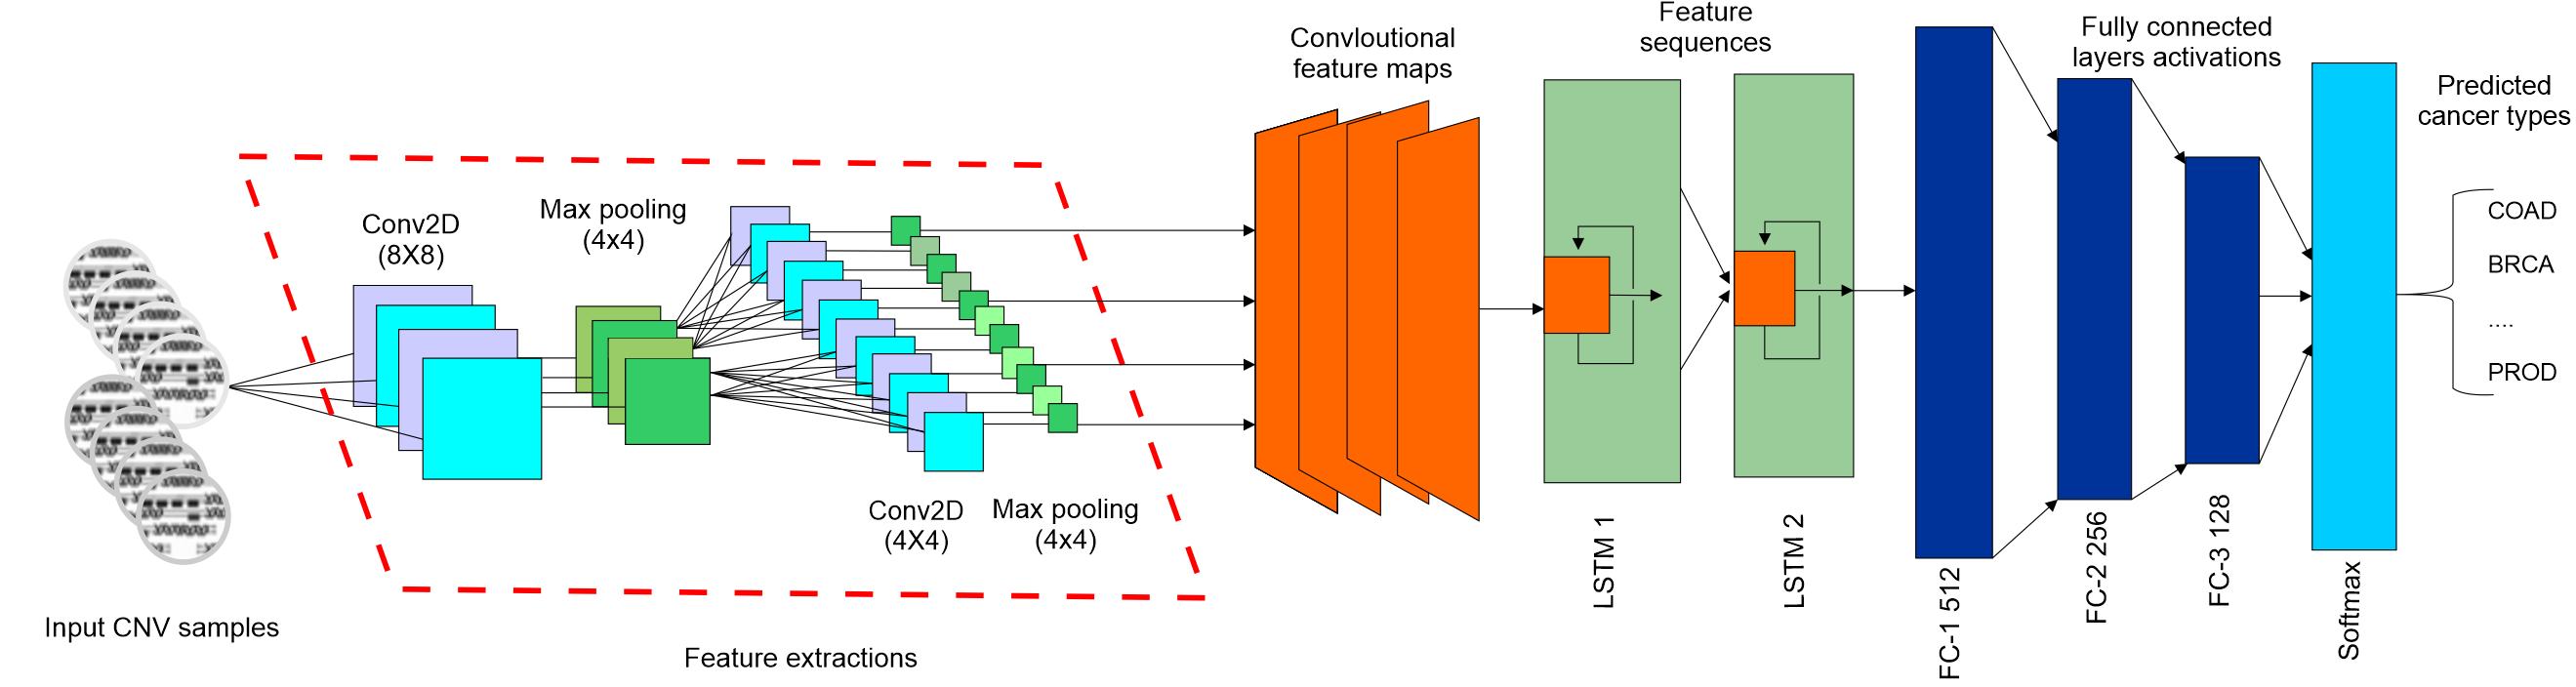
\includegraphics[scale=0.5]{images/conv_lstm.png} 
	\caption[Schematic representation of the convolutional-LSTM network]{Schematic representation of the CLSTM network starts from taking input CNV samples and passing to CNN layers before getting a sequence vector representation from the LSTM layers to pass to dense, dropout, and softmax layers~\cite{karimACCA2019}}	
	\label{fig:conv_lstm}
	\vspace{-2mm}
\end{figure*}

\hspace*{3.5mm} Output of each convolutional layer is then passed to the dropout layer to regularize learning to avoid overfitting~\cite{vardropout}. To down sample the input feature space into lower dimensional representation, two max pooling layer~(MPL) are placed with different filter size. The output of an MPL can be considered as an `extracted feature' from each CNV samples. Since each MPL follows to `flatten' the output space by taking the highest value in each timestep dimension, this helps produce a sequence vector, e.g., feature sequence from the last LSTM layer, which help the network to learn abstract features~(w.r.t. driver genes) that are highly indicative of being responsible for specific cancer type. This vector is then fed into the neural network  through another dropout and the softmax layers for the probability distribution over the classes. 

\subsubsection{Construction of CAE classifier}
Using the CLSTM-based network, we have seen how to extract both local and globally important features for classifying individual samples from a limited number of labelled samples. However, in cases of very small numbers of training samples, unsupervised pretraining has proven highly effective~\cite{ae1,ae2,ae3}. 
%\subsubsection{Handling data sparsity}
Humans communicate through languages or signs, which is analogous to biological organisms too, that convey information within and between cells through information encoded in biological sequences~\cite{yue2018deep}. To understand the language of life unsupervised data-driven representation learning methods such as BioVec~\cite{asgari2015continuous} is proposed. BioVec embeds biological sequences in lower dimensional vector space to characterizes biophysical and biochemical properties of sequences, and is already proven effective~\cite{yue2018deep}. 

\begin{figure*}[h]
	\centering
	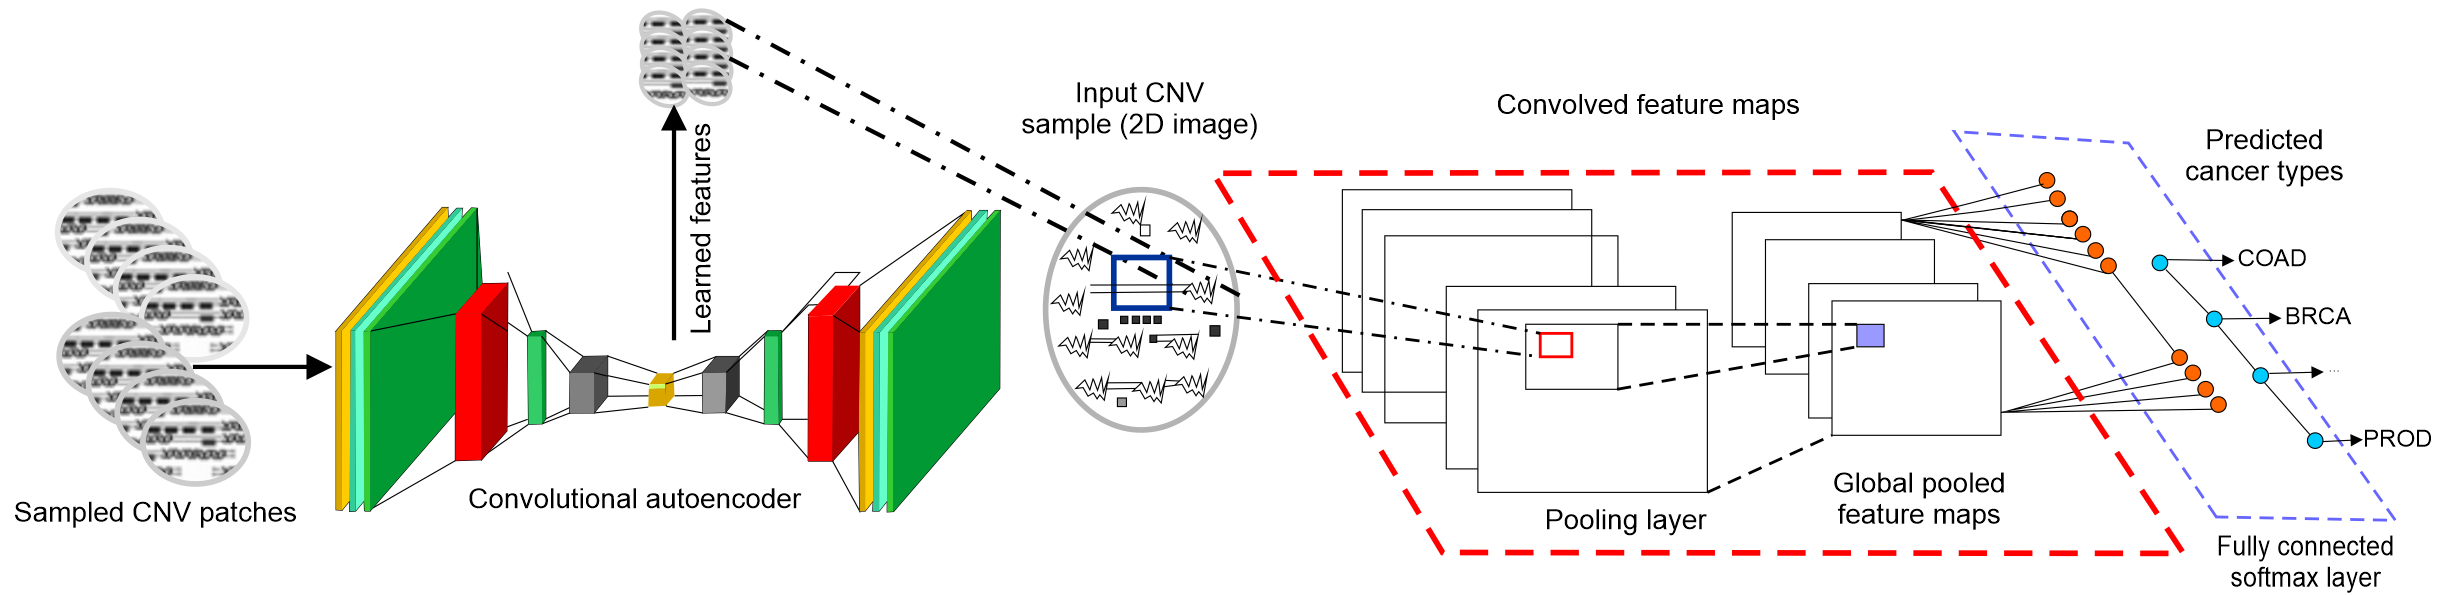
\includegraphics[scale=0.6]{images/cae.png}	
    \caption{Schematic representation of the CAE classifier~\cite{karimACCA2019}}
	\label{fig:cae}
\end{figure*}


\hspace*{3.5mm} Further, since both datasets are very sparse,  CAE-based representation learning is employed. Since sparse AEs are intrinsically sparse, it is important to apply sparsity constraints, e.g., self-regularization, with all the typical benefits associated with sparsity: it forces the model to focus on the really important features, highly reducing the risk of overfitting~\cite{karimBIB2019}. Especially, it is a major methodological guide for the correct tuning of the model capacity, progressively augmenting it to attain sparsity, or conversely reducing the dimension of the network removing links to zeroed out neurons~\cite{sparseAE}. 

\hspace*{3.5mm} Due to the sparsity of $L_1$ regularization, sparse AEs actually learns better representations such that the activation are sparser, which makes it perform better than an a regular AE without $L_1$ regularization as an AE learns latent representations instead of redundant information in our input data. 
%\subsubsection{CAE network construction}
A CAE is constructed, which is architecturally a 19-layer autoencoder, in which a batch normalization layer is used after every convolutional layer and the ReLu activation function in every layer except for last layer that uses a Softmax activation function. From the given CNV samples, feature map is calculated using convolutional layer in the encoder module. The pooling layer is calculated by down-sampling the convolutional layer by taking the maximum value in each non-overlapping sub-region. The CAE classifier contains of two parts -   autoencoder and the classifier. The autoencoder part has the following structure: 

\begin{enumerate}[noitemsep]
    \scriptsize{
        \item Input layer: each CNVs sample is reshaped from 1 x 20,736 to 144 x 144
        \item Convolutional layer: of size 32 x 20,736 (i.e. 144 x 144) 
        \item Batch normalization layer: of size 32 x 20,736
        \item Convolutional layer: of size 32 x 20,736
        \item Batch normalization layer: of size 32 x 10,368
        \item Max-pooling layer: of size 32 x 10,368
        \item Convolutional layer: of size 64 x 10,368
        \item Batch normalization layer: of size 64 x 10,368
        \item Convolutional layer: of size 64 x 10,368
        \item Batch normalization layer: of size 64 x 10,368
        \item Convolutional layer: of size 128 x 10,368
        \item Batch normalization layer: of size 128 x 10,368
        \item Convolutional layer: of size 128 x 10,368
        \item Batch normalization layer: of size 128 x 10,368
        \item Convolutional layer: of size 128 x 10,368
        \item Batch normalization layer: of size 128 x 10,368
        \item Convolutional layer: of size 64 x 10,368
        \item Batch normalization layer: of size 64 x 10,368
        \item Upsampling layer: of size 64 x 20,736 
        \item Convolutional layer: of size 1 x 20,736.}
\end{enumerate}

\hspace*{3.5mm} After training the CAE, the decoder component is removed by making the first 19 layers trainable false\footnote{Since the encoder part is already trained}. On top of these components, a flattening layer, followed by a fully connected dense layer of size 128 and a Softmax output unit of 14~(i.e., the number of classes) are added. 

\subsection{Network training and neural ensemble} %all human genes
Each of CLSTM and CAE is trained in two steps. Training is performed independently, followed by creating their multiple snapshots before applying MAE. Network parameters are initialized with Xavier initialization~\cite{xavier} and trained using AdaGrad - a first-order gradient-based optimization technique to optimize the categorical cross-entropy loss as: 

\vspace{-2mm}
\begin{equation} 
    E_{c} = \sum_{i, j, k} T_{i, j, k} \log P_{i, j, k}+\left(1-T_{i, j, k}\right) \log \left(1-P_{i, j, k}\right)
    \label{eq:cce3}
\end{equation} 

\begin{figure*}
    \centering
    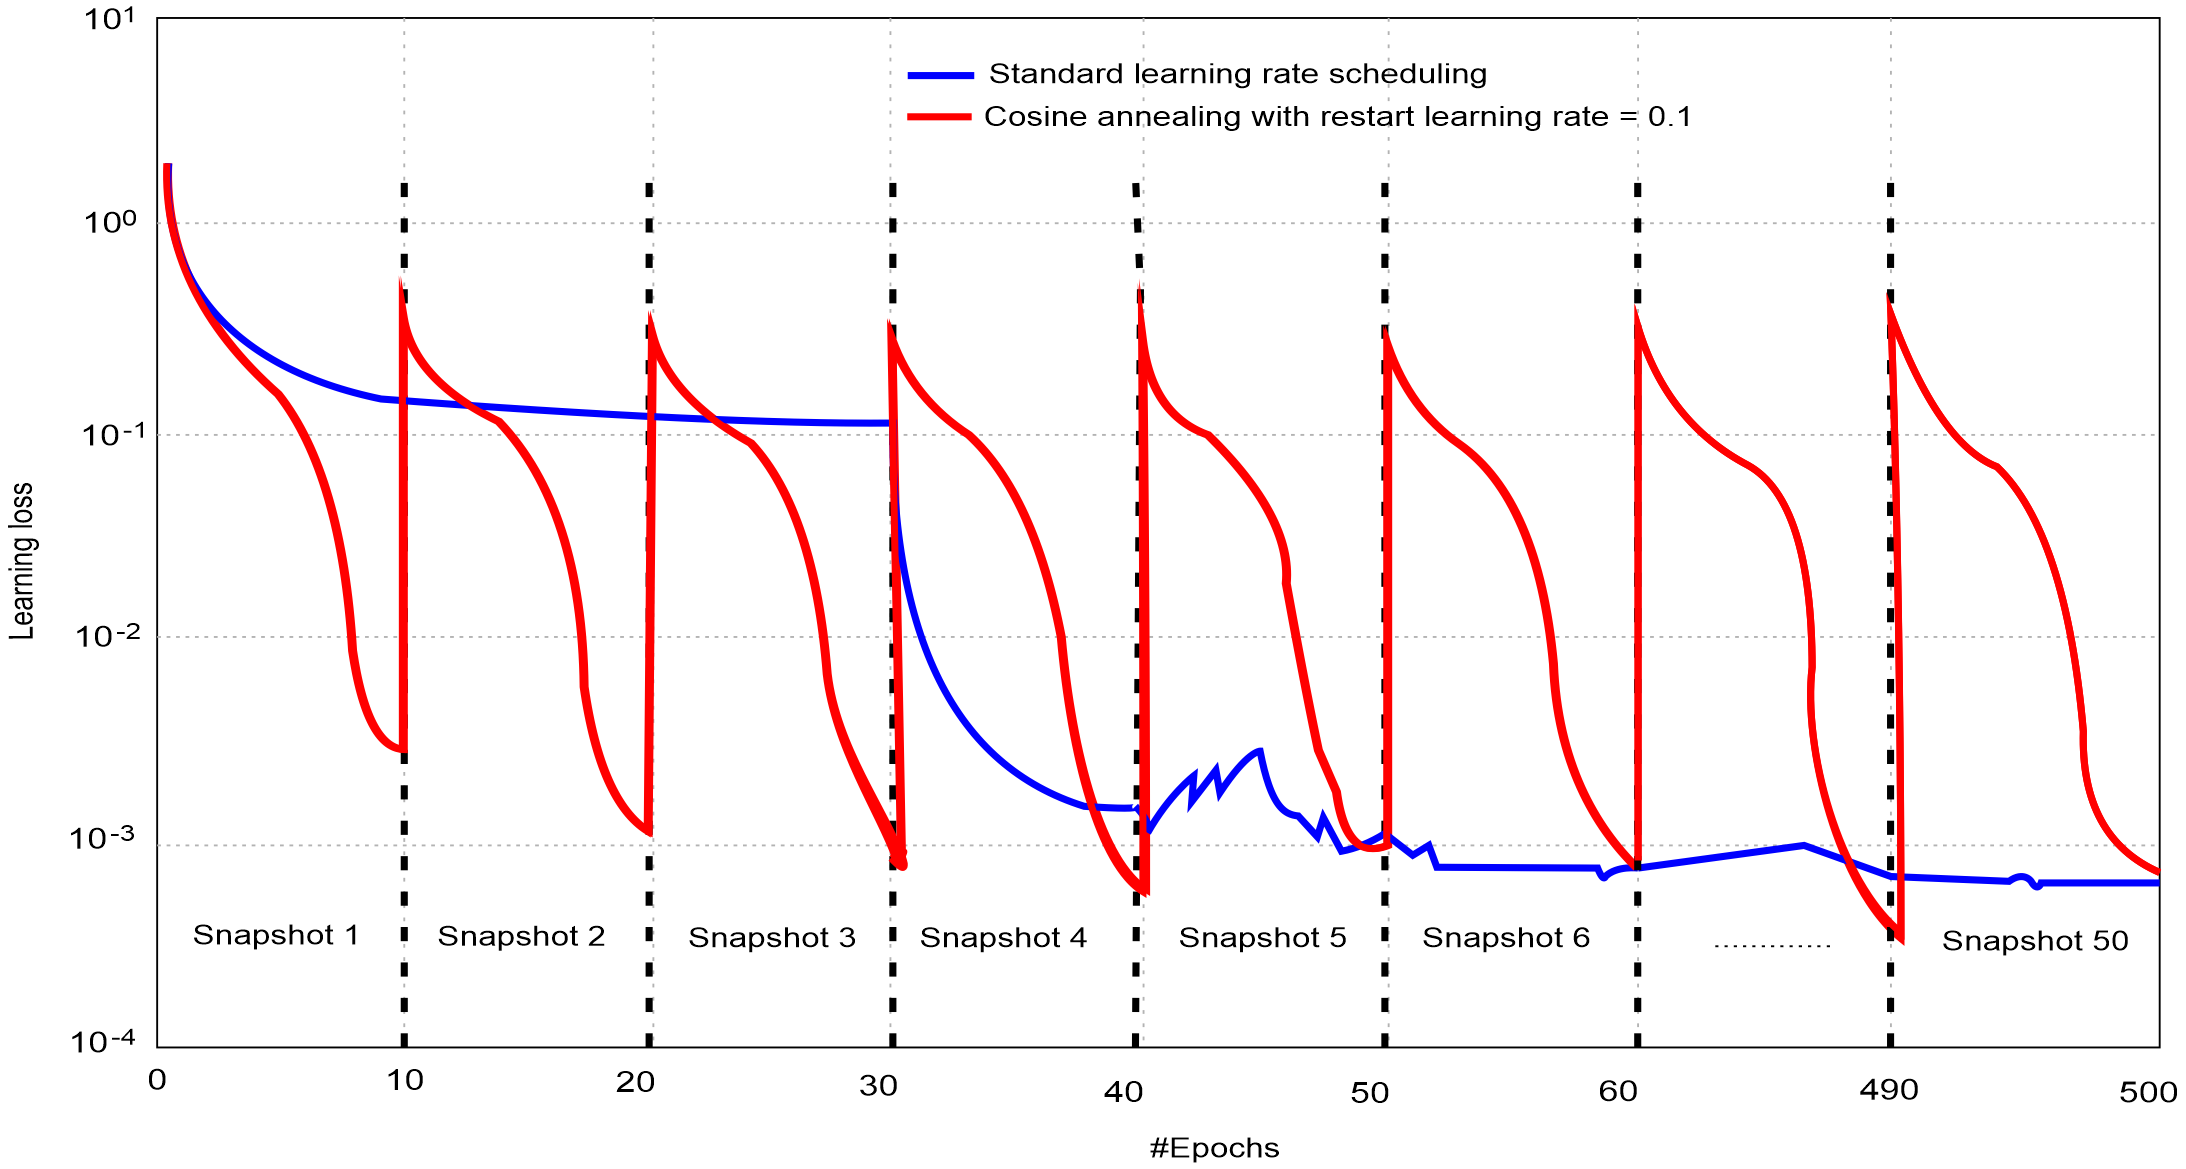
\includegraphics[scale=0.55]{images/cac.png}
    \caption[Cosine cyclic annealing-based training]{Training loss of CLSTM network with standard learning rate~(blue) vs. cosine annealing~(red): intermediate models~(denoted by the dotted lines) form an ensemble at the end of training~\cite{karimACCA2019}}
    \label{fig:ca}
    \vspace{-2mm}
\end{figure*}

\hspace*{3.5mm} Softmax activation function is used in the output layer for the probability distribution over the classes. Hyperparameters are defined in grid search and 10-fold cross-validation by varying learning rates and different batch sizes. Further, Gaussian noise layers are added, followed by convolutional and LSTM layers to improve model generalization and to reduce overfitting. 
%Model ensemble technique helps the neural network to achieve improved performance compared to the predictions from a single model by reducing the generalization error. 
%We hypothesize\footnote{\textbf{$H_3$:} A neural ensemble method, combining several deep architectures, can be more effective than structures solely based on a single model by reducing the generalization error~\cite{karimACCA2019}.} that a neural ensemble method by combining several deep architectures can be more effective than structures solely based on a single model~\cite{karimACCA2019}.
Cyclic cosine annealing~(CCA) is employed. CCA  aggressively~(but systematically) changes the learning rate~(LR) over epochs to produce different network weights~\cite{loshchilov2016sgdr}. Multiple model snapshots are created during a single training run and combine the predictions to make an ensemble prediction \cite{huang2017snapshot}. 

\hspace*{3.5mm} CCA requires total training epochs, maximum learning rate, and number of cycles, as well as the current epoch number making the initial LR and the total number of training epochs as two hyperparameters. Hence, CCA will have an effect of starting with a large LR, which is relatively rapidly decreased to a minimum value before being dramatically increased again to the following LR for the given epoch~\cite{huang2017snapshot}. CCA aggressively but systematically changes the learning rate over training epochs to produce very different network weights~\cite{loshchilov2016sgdr}, as outlined in~\cref{fig:ca}. 

\begin{equation}
    \label{eq:lr-cosine}
    \alpha(t)=\frac{\alpha_{0}}{2}\left(\cos \left(\frac{\pi \bmod (t-1,\lceil T / M\rceil)}{\lceil T / M\rceil}\right)+1\right)
\end{equation}

\begin{figure}
    \centering
        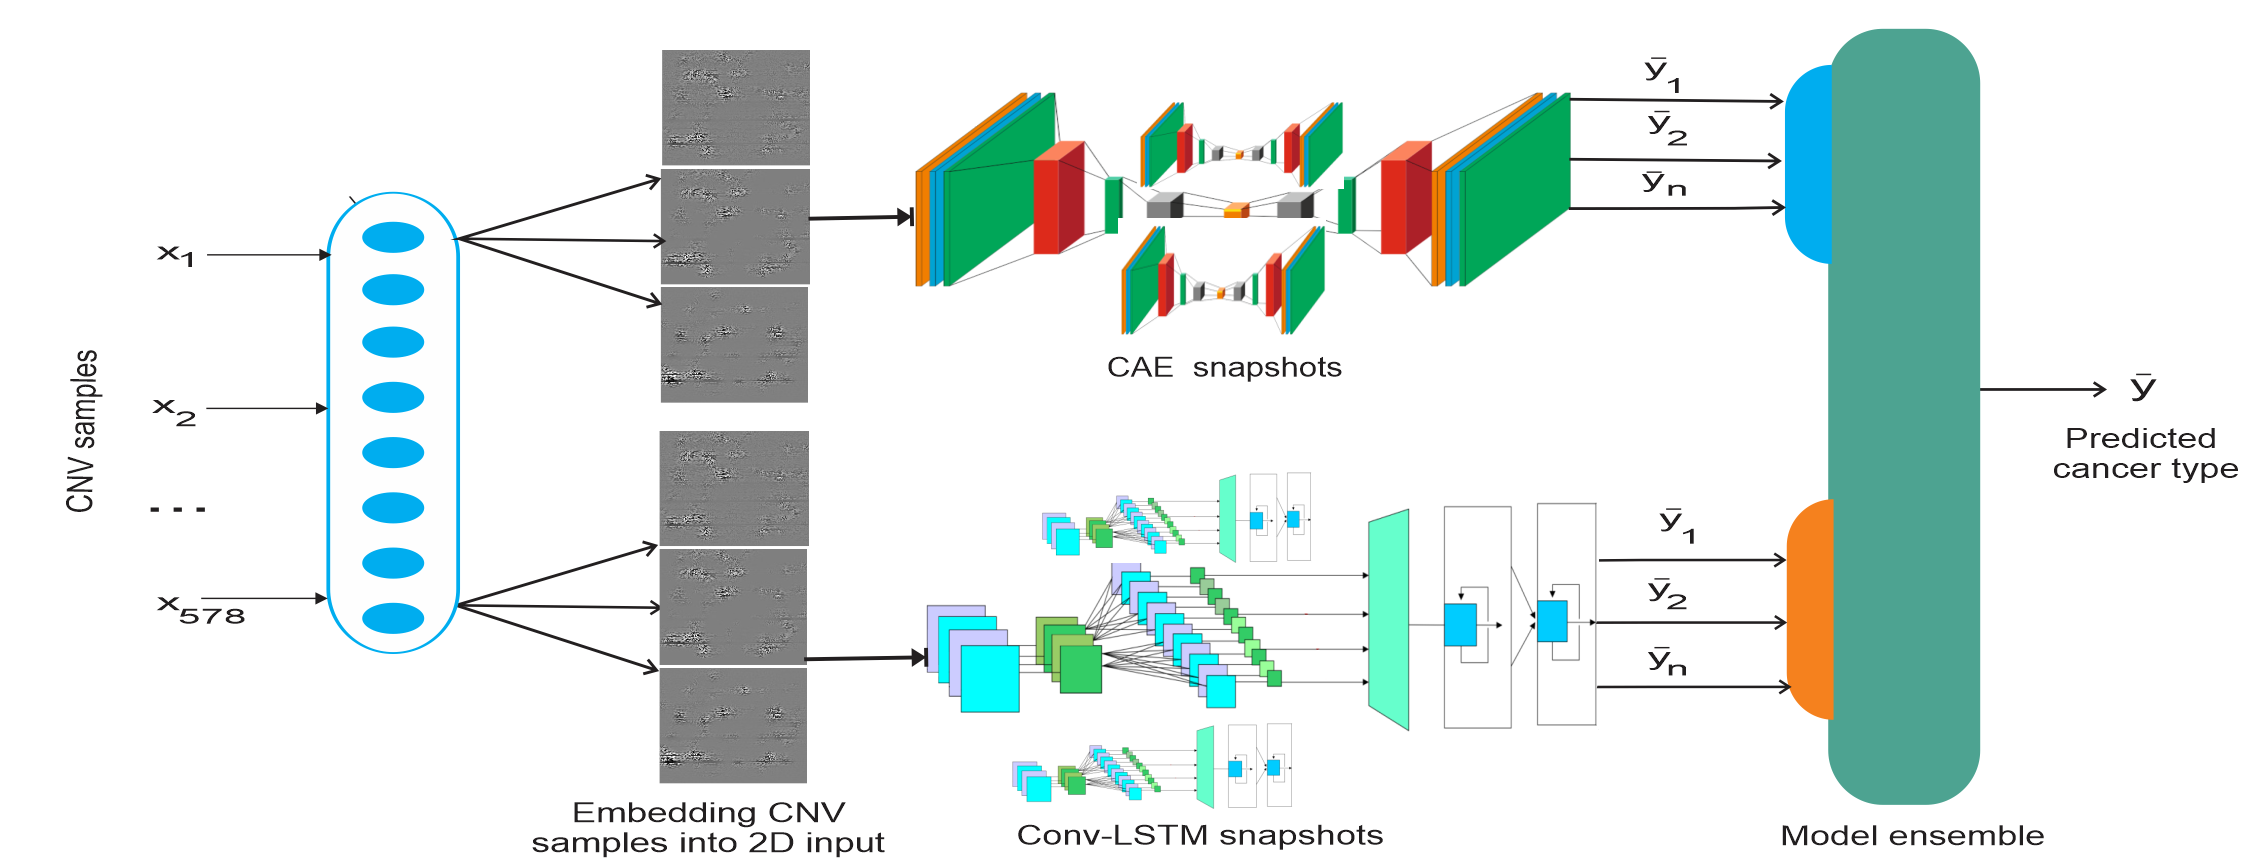
\includegraphics[scale=0.65]{images/ensemble.png}
    \caption{Model averaging ensemble of CLSTM and CAE snapshots~\cite{karimACCA2019}}
    \label{fig:mae}
    \vspace{-2mm}
\end{figure}

\hspace*{3.5mm} In \cref{eq:lr-cosine}, $\alpha(t)$ is the LR at epoch t, $\alpha_0$ is the maximum LR, $T$ is the total epoch, $M$ is the number of cycles, $mod$ is the modulo operation, and square brackets indicate floor operations. During the training of the ensemble model, we set total epochs, maximum learning rate, number of cycles, and current epoch number. Initial learning rate and total number of epochs are treated as hyperparameters. After training, best weights at the bottom of each cycle are saved as the snapshot of each model for $M$ cycles, giving $M$ model snapshots. Network undergoes several LR annealing cycles, converging to and escaping from multiple local minima during snapshot ensembling. The ensemble prediction is computed at test time, by averaging last $m$ model's Softmax outputs, where $m \leq M$, where $\mathbf{x}$ is a test sample and $h_i \left(\mathbf{x} \right)$ is the softmax score of snapshot $i$, the final output is the simple mean of the last $m$ models as follows~\cite{huang2017snapshot}: 

\vspace{-2mm}
\begin{equation}
    h_{\mathrm{MAE}}=\frac{1}{m} \sum_{0}^{m-1} h_{M-i}(\mathrm{x})
    \label{eq:mae}
\end{equation}

\hspace*{3.5mm} Finally, all the snapshot model are integrated and used in the final ensemble using MEA, as shown in \cref{fig:mae}. Although, each model's weights are subjected to dramatic changes during training for the subsequent LR cycles, CCA allows the learning algorithm to converge to a different solution. Subsequently, the ensemble model gives the lowest test error~\cite{huang2017snapshot}. %, since an exhaustive optimization would be too computationally expensive. %Further, we only use a single object property to test how results change with each choice of parameter, due to computational constraints. 

\section{Experiments}\label{chapter_3:results}
Several experiments were carried out based on protein-coding genes and oncogenes. By using each network and CNV representation, cancer type predictions were evaluated separately, with the following objective:

\begin{enumerate}[noitemsep]
    \item Which neural network architecture is more suitable for handing high dimensional CNV data. 
    \item Does neural ensemble method can outperform single and standalone model.
    \item Does CNV is biological suitable for cancer subtyping task? 
\end{enumerate}

\hspace*{3.5mm} Results of each observation are analysed, both quantitative and qualitatively, in the following section. 

\subsection{Experiment setup}
Parameters for the individual model is first optimized, followed by the same for the ensemble model. During the training of CLSTM and CAE, 70\% of the data is used for the training, 30\% for the evaluation, and 10\% from the training set to optimize the learning rate, batch size, number of filters, kernel size, dropout probability, and Gaussian noise probability. For pretraining the CAE, 90\% of data is used for the training, and 10\% of the data is used for validation. 
During the ensemble training, number of epochs~(NE), maximum learning rate, and number of cycles~(NC), are set to 500, 1.0, and NE/10, respectively, for each model for 50 cycles through a grid search, giving 50 snapshots. 

\hspace*{3.5mm} Results based on best hyperparameters produced through random search and 5-fold cross-validation tests empirically are reported in a macro-averaged precision and recall setting as classes are imbalanced. F1-scores are not reported since it is significant only when the value of precision and recall are very different. Nevertheless, for cancer diagnosis, it is important to have both high precision and recall. Hence, results with very different precision and recall are not useful in cancer diagnosing and tumor type identification. Besides, confusion matrices for both CLSTM and CAE models are interpreted. 
%The MAE is then followed to report the final predictions. 

\subsection{Performance analysis of individual models}
Classification accuracies using oncogenes and all protein-coding genes vary. In particular, using protein-coding genes, classifiers perform moderately well, giving accuracies of 72.96\% and 76.77\% with CLSTM and CAE network, respectively. Since classes are imbalanced, accuracy alone gives distorted estimation of the cancer types. Thus, class-specific classification reports are shown in \cref{table:codingene} and \cref{table:resultoncogene}. As shown in~\cref{table:codingene}, precision and recall for majority cancer types were moderately high in which CAE performed mostly better than CLSTM network. In particular, CAE classifier can classify COAD, GBM, KIRC, BRCA, LUSC, and PRAD more confidently~(at least 82.50\% of the cases); CLSTM classified the OV tumor samples more accurately than CAE classifier~(83.56\% vs 76.13\%). 

\begin{table} [h]
\caption{Performance on cancer type prediction using protein-coding genes}
\label{table:codingene} %RF Confusion Matrix all genes Subtype
    \begin{center}
        \vspace{-5mm}
    \scriptsize
        \begin{tabular}{l|ll|ll|l}
        \hline
        \rowcolor{Gray}
        {} & \multicolumn{2}{c}{\textbf{CLSTM~(72.96\%)}} & \multicolumn{2}{c}{\textbf{CAE~(76.77\%)}} &  {} \\\hline
        \textbf{Tumor type} & \textbf{Precision} &  \textbf{Recall}  & \textbf{Precision} &  \textbf{Recall} & \textbf{Support} \\\hline
        COAD    & 0.6981  &  0.7325 & 0.7924 &    0.8250 & 133  \\\hline
        GBM     & 0.8127  &  0.8275 & 0.8247 &   0.8765  & 151  \\\hline
        KIRC    & 0.8013  &  0.7335 & 0.8331 &   0.8468  & 150  \\\hline
        LGG     & 0.8250  &  0.6935 & 0.8642 &   0.7835 & 120  \\\hline
        LUAD    & 0.6835  &  0.6584 & 0.6992 &   0.7238 & 136  \\\hline
        LUSC    & 0.6937  &  0.7294 & 0.7438 &   0.8352 & 132  \\\hline
        OV      & 0.7539  &  0.8356 & 0.8365 &   0.7613 & 145  \\\hline
        UCEC    & 0.6645  &  0.6829 & 0.7435 &   0.6834 & 131  \\\hline
        BRCA    & 0.7357  &  0.7587 & 0.7954 &   0.8386 & 269  \\\hline
        HNSC    & 0.7134  &  0.7235 & 0.6853 &   0.7542 & 141  \\\hline
        THCA    & 0.6967 &  0.6959 & 0.7025 &   0.7654 & 121  \\\hline
        PRAD    & 0.7225  &  0.7934 & 0.8395 &   0.8345 & 124  \\\hline
        STAD    & 0.6528  &  0.6917 & 0.6776 &   0.6512 & 113  \\\hline
        BLCA    & 0.7356  &  0.6589 & 0.7925 &   0.7489 & 108  \\\hline
        \rowcolor{LightCyan}
        \textbf{Avg/total} & \textbf{0.7278} &    \textbf{0.7296} & \textbf{0.7593} &    \textbf{0.7677} & \textbf{1974}  \\\hline
        \end{tabular}
        \vspace{-4mm}
    \end{center}
\end{table}

\hspace*{3.5mm} The downside is that both classifiers have made a substantial amount of mistakes e.g., CAE can classify STAD and UCEC tumor cases only 65\% and 68\% accurately; CLSTM network made more mistakes particularly for the STAD, BLCA, THCA, UCEC, LUAD, and LGG tumor samples. On the other hand, although the tumor-specific classification accuracies varied across classes, the overall accuracies increased moderately and reached 74.25\% and 78.32\% using CLSTM and CAE, respectively. As seen in~\cref{table:resultoncogene}, the precision and recall for most of the cancer types are higher than that of protein-coding gene-based CNVs. Similar to the previous experiment, CAE performed mostly better than the CLSTM network across tumor types. In particular, CAE classifier can correctly classify COAD, GBM, OV, UCEC, PRAD, and BLCA in at least 80\% of the cases showing higher confidence. 

\begin{figure}[h]
	\centering
	\begin{subfigure}{0.48\linewidth}
		\centering
		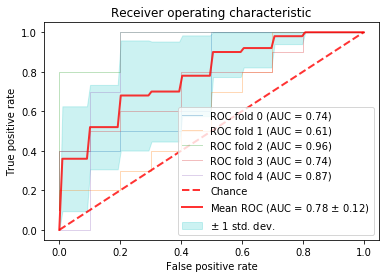
\includegraphics[scale=0.55]{images/download1.png}
		\caption{Using CAE classifier}
	\end{subfigure}
	\hspace{2mm}
	\begin{subfigure}{0.48\linewidth}
		\centering
		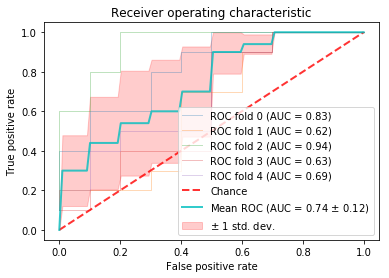
\includegraphics[scale=0.55]{images/download2.png}
		\caption{Using CLSTM network}
	\end{subfigure}
	\caption{The ROC curves for CLSTM and CAE models across folds} 
	\label{fig:roc}
	 \vspace{-2mm}
\end{figure}

\begin{table}[h]
\caption{Performance on cancer type prediction using oncogenes }
\label{table:resultoncogene} 
\begin{center}
    \scriptsize
    \vspace{-5mm}
    \begin{tabular}{l|ll|ll|l}
        \hline
        \rowcolor{Gray}
        {} & \multicolumn{2}{c}{\textbf{CLSTM (74.67\%)}} & \multicolumn{2}{c}{\textbf{CAE (78.32\%)}} &  {} \\\hline
        \textbf{Tumor type }& \textbf{Precision} &  \textbf{Recall}  & \textbf{Precision} &  \textbf{Recall} & \textbf{Support~(CAE)} \\\hline
        COAD   & 0.7785 & 0.7564 & 0.8265 & 0.8193 & 133  \\\hline
        GBM    & 0.8254 & 0.8330 & 0.8433 & 0.8524 & 151  \\\hline
        KIRC   & 0.7753 & 0.7835 & 0.8172 & 0.8035 & 150  \\\hline
        LGG    & 0.8235 & 0.7136 & 0.7976 & 0.8031 & 120  \\\hline
        LUAD   & 0.7520 & 0.7351 & 0.7584 & 0.7674 & 136  \\\hline
        LUSC   & 0.7528 & 0.6475 & 0.7139 & 0.7256 & 132  \\\hline
        OV     & 0.8327 & 0.8407 & 0.8665 & 0.8538 & 145  \\\hline
        UCEC   & 0.7726 & 0.7625 & 0.8732 & 0.8412 & 131  \\\hline
        BRCA   & 0.7956 & 0.8075 & 0.8012 & 0.7965 & 269  \\\hline
        HNSC   & 0.8253 & 0.6932 & 0.7025 & 0.6929 & 141  \\\hline
        THCA   & 0.7953 & 0.8025 & 0.7429 & 0.7581 & 121  \\\hline
        PRAD   & 0.8267 & 0.8237 & 0.8781 & 0.8626 & 124  \\\hline
        STAD   & 0.7924 & 0.6945 & 0.7632 & 0.7737 & 113  \\\hline
        BLCA   & 0.8368 & 0.7979 & 0.8623 & 0.8553 & 108  \\\hline
        \rowcolor{LightCyan}
        \textbf{Avg/total} &   \textbf{0.7543}    &  \textbf{0.7467} &    \textbf{0.7945}   &  \textbf{0.7832} & \textbf{1974} \\\hline
    \end{tabular}
     \vspace{-6mm}
    \end{center}
\end{table}

\hspace*{3.5mm} On the contrary, CLSTM classified the BRCA and THCA tumor samples more accurately than the CAE classifier. The downside is that both classifiers have made substantial mistakes, too. For example, CAE could classify HNSC and LUSC tumor samples accurately in only 69\% and 72\% of the cases. Whereas, the CLSTM network made more mistakes, particularly for the STAD, HNSC, LUSC, and LGG tumor samples. In summary, both classifiers performed moderately well except for certain types of tumor cases such as STAD, HNSC, BLCA, THCA, UCEC, LUAD, LUSC, and LGG. The ROC curves in \cref{fig:roc} based on CNVs from oncogene shows that AUC scores generated by both the CLSTM model and CAE classifier are consistent across folds, and AUC scores generated by the CAE classifier are about 4\% better than that of the CLSTM network.

\begin{figure}[h]
	\centering
	\begin{subfigure}{0.48\linewidth}
		\centering
		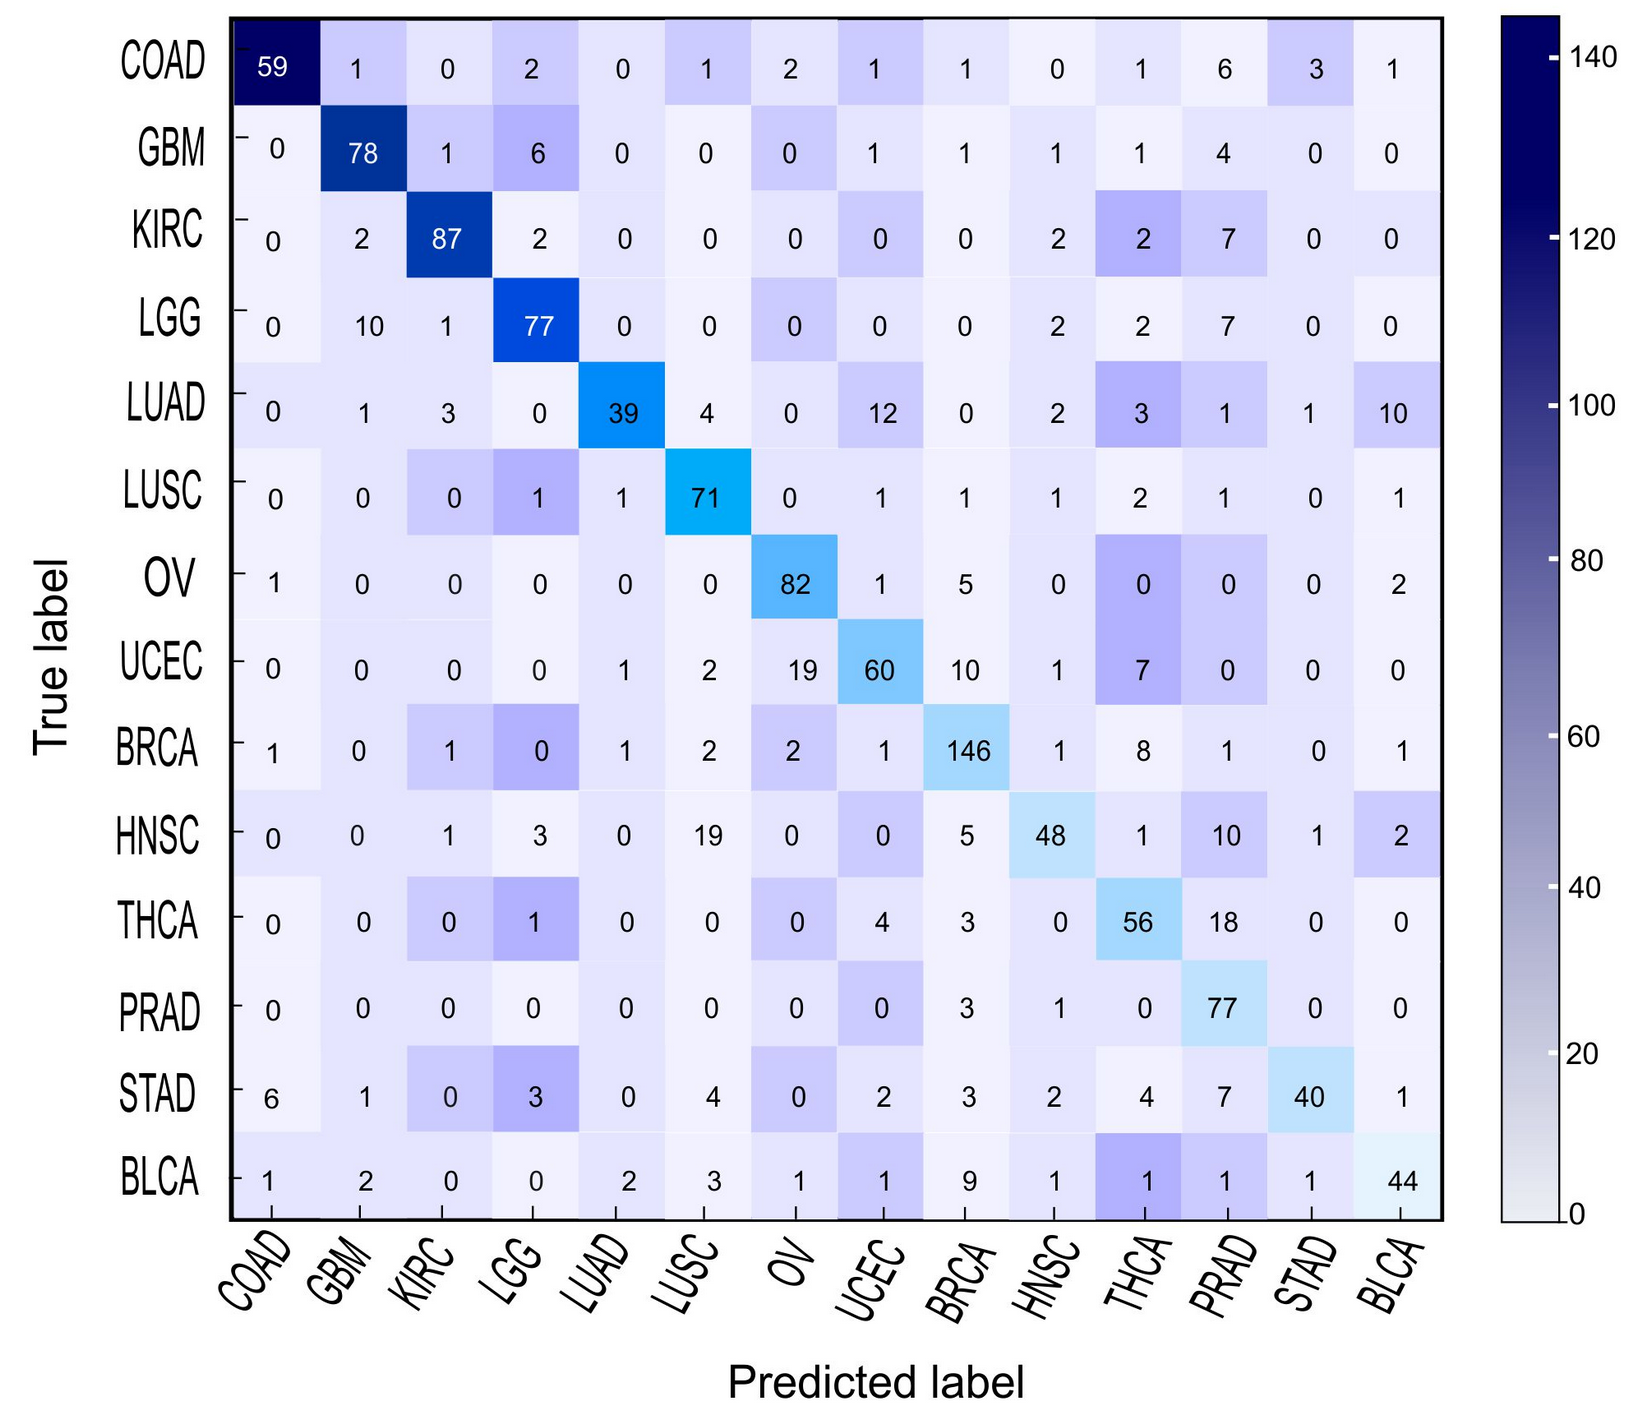
\includegraphics[scale=0.35]{images/cm1.png}
		\caption{Using coding genes based CNVs}
        \label{fig:cm_1}
	\end{subfigure}
	\hspace{2mm}
	\begin{subfigure}{0.48\linewidth}
		\centering
		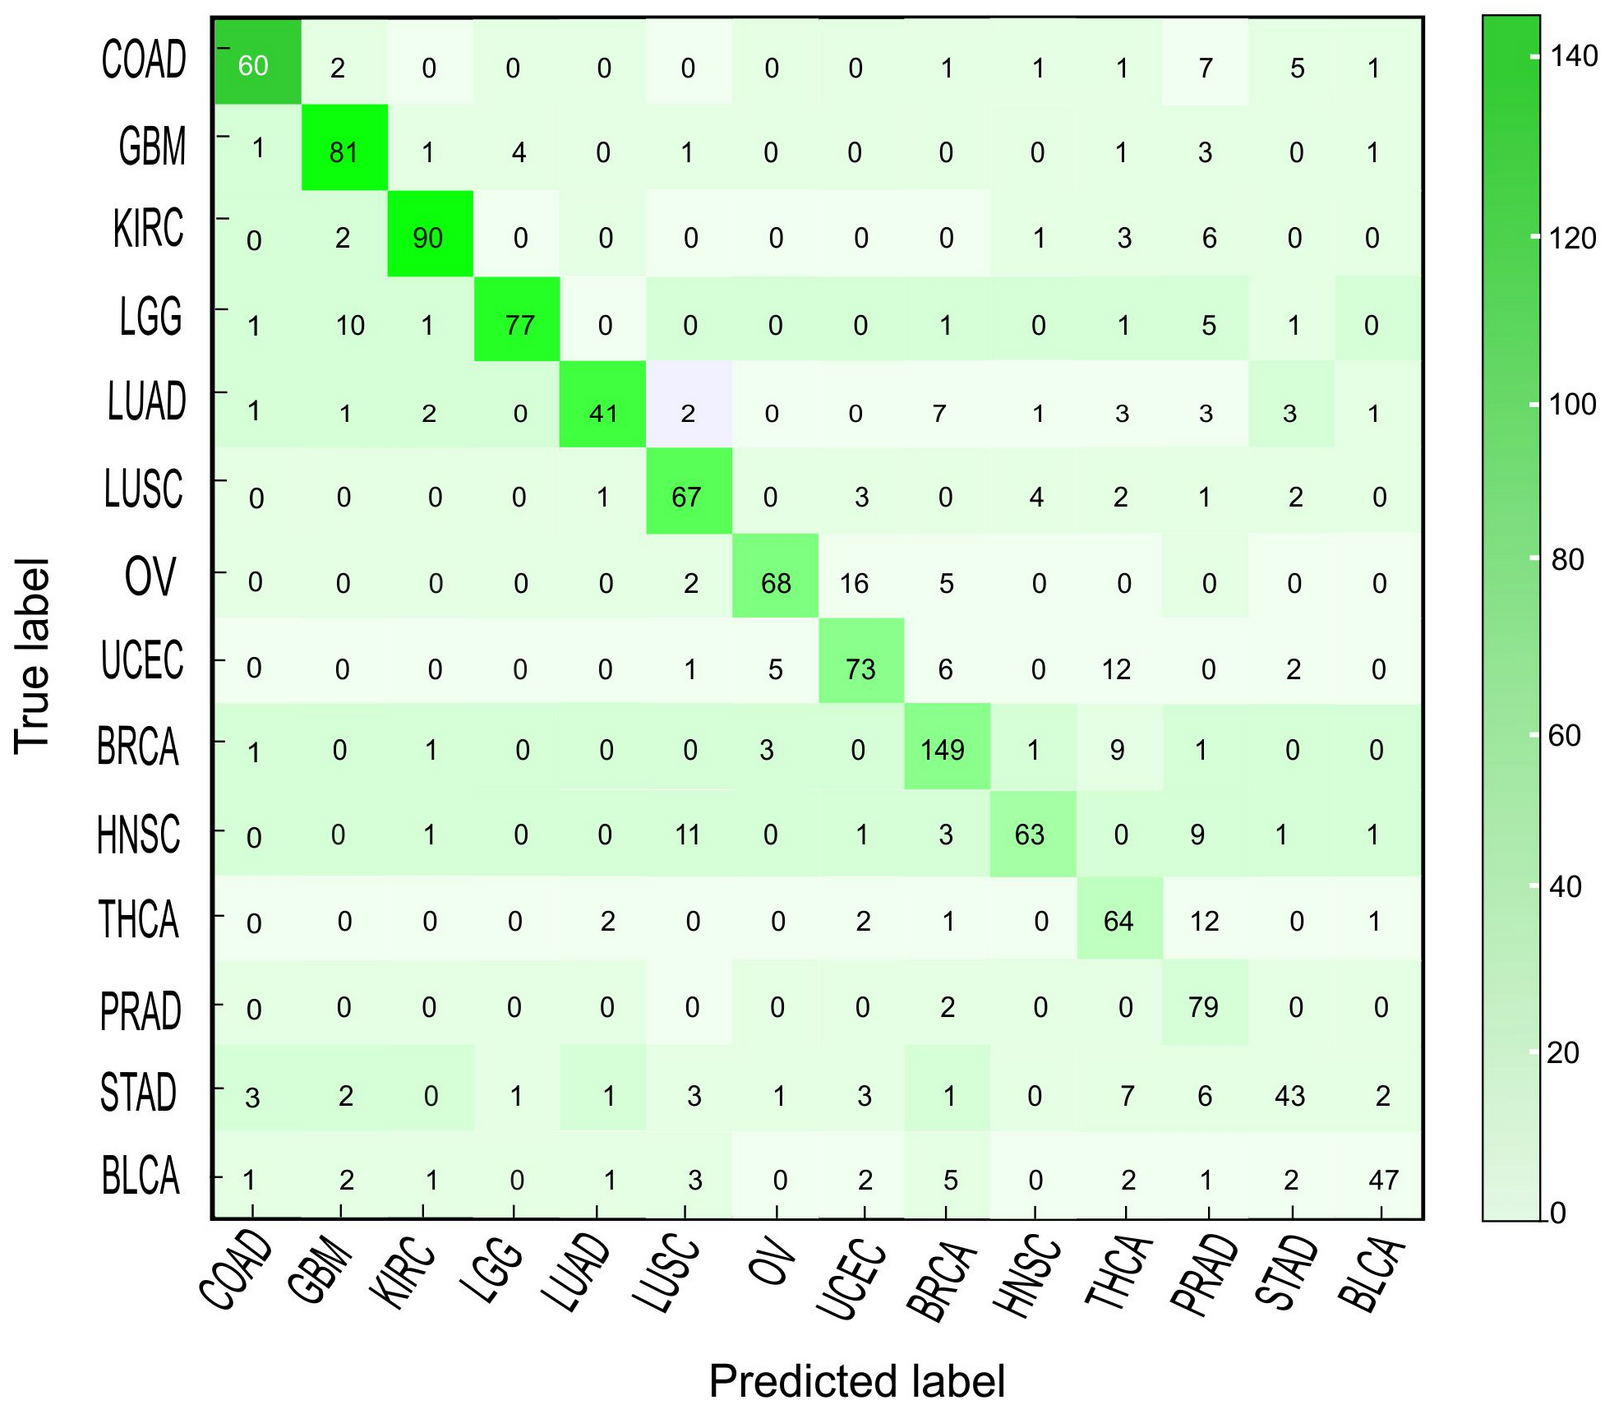
\includegraphics[scale=0.35]{images/cm2.png}
		\caption{Using oncogenes based CNVs}
        \label{fig:cm_2}
	\end{subfigure}
	\caption{Confusion matrices of the ensemble classifier} 
	\label{fig:cms}
	 \vspace{-4mm}
\end{figure}

\subsection{Performance analysis of the ensemble model}
The ensemble classifier shows about 4\% and 2\% performance boost across classes and overall in the cases of oncogenes and protein-coding gene-based experiment, respectively. The accuracy looks easy enough but makes no distinction between classes e.g., when a doctor makes a medical diagnosis that a patient has cancer, but in reality, the patient does not~(i.e., false positive). This has very different consequences than making the call that a patient does not have cancer when he actually does~(i.e., false negative). A more detailed breakdown of correct and incorrect classifications for each class using the confusion matrices is shown in \cref{fig:cms}, which correspond to ground truth labels vs. the predictions made.

\hspace*{3.5mm} There are significant accuracy improvements in case of STAD, HNSC, BLCA, THCA, UCEC, and LUSC tumor types. In case of UCEC and LUSC cancer types, not only are the accuracies increased slightly, but also the false positive rates are reduced significantly. On the contrary, using oncogenes, the classifiers were less confused among tumor types, except for the LGG, HNSC, and THCA tumor types. Despite these improvements, there is still high confusion among LUAD, HNSC, and LGG samples, which is because features from these tumor samples are highly correlated. We could not find an exact reason for such behavior. Perhaps, a more gene-specific CNV analysis is required to confirm such correlations. However, poor and imbalance training might be one of the reasons. 

\section{Discussion}\label{chapter_3:discussion}
Some previous studies~\cite{zhang2016classification,elsadek2018supervised} that focused on using CNV based cancer typing method used data from cBioPortal. They applied incremental feature selection methods before training classic ML models and managed to achieve classification accuracy of 75\% and 85\%~(by Zhang et al. and Sanaa F. et al., respectively). Since we have more samples and from different sources, a one-to-one comparison was not viable. Still, the ensemble model achieved about a classification accuracy of 80\%, which is about 6\% better than our previous approach~\cite{karim2018a2ic} w.r.t. every metric. 

\hspace*{3.5mm} However, considering an accuracy of 80\%, we cannot claim that our model’s confidence is very high. This is for several reasons, such as lack of training samples, poor training, and data sparsity. The latter reason caused each network to produce high training and validation loss of error optimization during the training phase, giving lower accuracy. Data sparsity was an issue too. In particular, on average, only 422 samples per tumor were used for the training, which is fairly low for such high-dimensional data. As a result, models are not able to identify subtle differences among tumor types. 
%We lacked enough training samples compared to the complex dataset, as deep architectures usually expect more samples to get trained well. %For the same reason, there was a lack of samples to perform model validation during 5-fold cross-validation. 
Another reason for poor training might be an imbalanced dataset. Some cancer types, such as BRCA, have 2.5 times more samples than other tumors. For example, STAD and BLCA have at least 15\% sample difference with other tumor types. These two tumors have very low classification accuracy, where about half of the samples were misclassified. Further, due to stochastic nature, ML algorithms are tend to produce different results. Besides, depending on the genome sequencing and CNV calling tools, different copy numbers might produce, with different CNV lengths and segmentation means, giving different results.

\section{Chapter Summary} \label{chapter_3:conclusion}
In this chapter, a snapshot neural ensemble method is developed for cancer-type prediction based on CNVs data using two deep architectures called CLSTM and CAE. The snapshot model training is based on cyclic cosine annealing technique, which create multiple model snapshots of these networks, followed by MAE technique to combine the predictive power of these architectures.  

%Another type of data~(e.g., DNA methylation, gene or miRNA expression, etc.) can be used to create a multimodal network in a similar fashion of single modality-based cancer typing method. %Downside of this single modality-based cancer typing method is that the findings are not validated with other annotations or scientific literature, which is why it cannot confirm if the identified genes are biologically relevant. Besides, it is not clear how the output is traced back to the inputs, nor it is clear why the outputs are transformed the way they are. Therefore, both models are `black-box'. %\hspace*{3.5mm} On the other hand, along with accurate identification of cancer types and most relevant biomarkers are the prerequisites for an oncologist to recommend more accurate treatments and drug repositioning. The latter only can be achieved with meaningful explanations, which helps healthcare experts to make reasonable and data-driven decisions to provide personalized diagnosis~\cite{stiglic2020interpretability}.  

\hspace*{3.5mm} CLSTM and CAE classifiers can classify patient cohorts with a precision of 0.7278 and 0.7593, respectively based on feature representation from protein-coding genes. Based on feature representation from oncogenes, CLSTM and CAE classifiers can classify patient cohorts with a precision of 0.7543 and 0.7945, respectively. Although the diagnosis accuracy is fairly low for both CAE and CLSTM classifiers, CAE classifier outperformed CLSTM network for all the experiments. To summarize, this chapter disseminate the following findings, through several experiments:  

\begin{enumerate}[noitemsep]
    \item \textbf{Does CNV is biological suitable for cancer subtyping task?} - experiment results show that CNVs are not only useful for predicting certain types of cancer, but also demonstration association with cancer growth. This suggests that CNV data is fairly suitable for the diagnosis of cancer. 
    \item \textbf{Which neural network architecture is more suitable for handing high dimensional CNV data?} - CAE classifier that learn latent CNV representation based on CAE autoencoder found to be more effective than CLSTM architecture. This suggests that CNN architectures could be more effective for high dimensional genomics data.   
    \item \textbf{Does neural ensemble method can outperform single and standalone model?} - the ensemble classifier shows about 2 to 4\% performance boost across classes and overall in the cases of protein-coding and oncogenes-based experiment, respectively. 
\end{enumerate}

\hspace*{3.5mm} Further, since multiple factors are involved in accurate cancer diagnosis, e.g., estrogen receptor~(ER), progesterone receptor~(PGR), and human epidermal growth factor receptor 2~(HER2/neu) statuses for breast cancer, providing AI-based diagnoses solely based on CNVs may not be reliable. From the carcinogenics point of view, multimodal features representation from DNA methylation, GE, miRNA expression, and CNVs data is required. 
%Lastly, a DL approach using CNV data along with other types of genomics data from different cohorts such as DNA methylation, GE, and mutations will be more reliable. 
In the next chapter, this work will be extended by increasing the number of samples for training, testing, and validation, by combining samples from Pan Cancer Atlas. A multimodal neural network architecture will be constructed and trained to combine features interpret the combinations to predict the cancer subtypes. 
